\documentclass[12pt]{article}
\usepackage{verbatim}
\usepackage[dvips]{epsfig}
\usepackage{color}
\usepackage{url}
\usepackage[colorlinks=true]{hyperref}

\begin{document}

\section*{GENESIS: Documentation}

{\bf Related Documentation:}
% start: userdocs-tag-replace-items related-do-nothing
% end: userdocs-tag-replace-items related-do-nothing

\section*{Technical Guide 1}

  This documents introduces the modular components of GENESIS 3.
  Following installation of the Neurospaces project packages
  (www.neurospaces.org), this document may be consulted as a user
  tutorial. It illustrates how to construct a biophysically realistic
  single compartment neuron from a {\tt swc} neuron morphology file.
  This tutorial may be usefully read in conjunction with [1, 2].

\section{Introduction}
GENESIS 3 (G3) has been
developed following the Computational Biology Initiative (CBI)
simulator functional architecture described in [1]. That document
specifies a software architecture appropriate for a neuronal
simulator. In such a simulator the layers of the software architecture
naturally correspond to high- and low level data, or biological
concepts and numerical values, respectively. One consequence of this
approach is that each software component in the architecture is
self-contained and can be run stand-alone. In this sense the CBI
architecture describes a highly modular system that provides a radical
departure from currently available neuronal simulation packages. Those
packages are typically monolithic and expose an arbitrary mixture of
biological and mathematical detail to the mathematical solvers and
users. In comparison with such packages, the data layering employed by
the G3 architecture clearly separates the mathematical details from
the biological framework required for a computational model. Thus, the
CBI functional simulator architecture has several important practical
consequences. For the developer, it greatly reduces the tremendous
complexity of dealing with a whole simulator, and for the modeller it
greatly increases the usability of the mathematical solvers.

In this section we introduce the major components of the Neurospaces
instantiation of G3 (NS) which includes: Neurospaces Model Container
(NMC) itself, and the Simple Scheduler in Perl (SSP). For completeness
we mention Heccer, the G3 mathematical solver and Neurospaces Studio
(NSS), the NS browser and visualization tool. It is assumed that these
modules have been installed on your computer. We will then lead you
through the process of how they can be used to build a single
biophysically realistic neuron model and simulation. The aim is to
introduce the declarative programing at the root of the G3 simulator
and develop an intuition for the practical development of G3
applications. Examples are given in the relevant sections below.

\subsection{Neurospaces Model Container}
\label{sec:neur-model-cont}
The Neurospaces Model Container (NMC) is the software component of NS
that reads definitions of a biological model from source files, stores
these data in memory, and translates them to the required mathematical
entities.

In concordance with the CBI simulator functional architecture, the NMC
is a stand-alone application that can be linked to GENESIS.  The NMC
deals purely with the biological entities and end-user concepts
of a biophyscally realistic model rather than the mathematical
equations that describe a model.  It separates biological, physical
and mathematical quantities of a simulation and 'knows' about
biological entities such as neuronal populations, single neurons, and
their projections and connections.  It also stores specific parameter
values obtained from the literature as well as the actual parameter
values employed during the simulation of a model.  Functionally, the
NMC is aware of neuronal morphology, membrane, and intracellular
components such that the biological objects it contains rely
hierarchically on their parents, children, and sibling's parameters to
infer a number of their own properties.

\subsection{Neurospaces Studio}
Neurospaces Studio (NSS) is a front-end to the NMC but is not a
graphical editor or neuron construction kit. (External applications
such as {\it neuroConstruct}, www.neuroconstruct.org, are more suited
for that type of functionality.) Rather, NSS allows browsing,
visualization, and validation of model parameters.

\subsection{Heccer}
{\it Heccer} (HEC) is a fast compartmental solver based on the {\it
  hsolve} functionality of the GENESIS simulator.

\subsection{Simple Scheduler in Perl}
The role of the Simple Scheduler in Perl (SSP) is to activate other
stand-alone G3 software components according to a configurable
schedule. SSP `glues' together these independent modules to ensure
that they are activated correctly, such that they can work together on
a single simulation.
 
\section{Introduction to Neurospaces}
This section contains general introductory comments about getting
started with NS.

\subsection{Neurospaces Model Descriptions}
A Neurospaces Model Description File (NDF) is the file format used to
specify models, from those of intracellullar mechanisms to network
models and morphologies.  The file format is indicated by {\tt .ndf}
being appended to the name of a regular text file, e.g. {\tt
  <filename>.ndf}.

It is possible to convert neuron morphology files to {\tt .ndf} files
using the command {\tt morphology2ndf} (see
section~\ref{sec:morph-conv-conf}).  A GENESIS script interface is
currently under construction.  This interface will allow to run
GENESIS scripts and execute the simulation, or simply convert the
model specified by the GENESIS scripts to Neurospaces model
descriptions.

A step-in example of consructing an NDF file can
be found in section~\ref{sec:simple-single-comp}.


\subsection{Overview of a NDF File}
\label{sec:overview-ndf-file}
A NDF file contains four sections. These sections are not necessarily
filled, but they must be present in the given order.  A NDF file has
the following general form which is described in the sections below.

\begin{center}
  \begin{minipage}{13cm}
\begin{verbatim}
#!/usr/local/bin/neurospacesparse
//-*- NEUROSPACES -*-

// default location for file comments

NEUROSPACES NDF

IMPORT
   FILE <namespace> "<directorypath>/<filename.ndf>"
   . . . <other files may be imported as required>

END IMPORT

PRIVATE_MODELS
   ALIAS <namespace>::/<source label> <target label> END ALIAS
   . . . <other aliases may be defined as required>

END PRIVATE_MODELS

PUBLIC_MODELS
   CELL <morphology name>
      SEGMENT_GROUP segments
         . . . <morphological details>
      END SEGMENT_GROUP
   END CELL
END PUBLIC_MODELS
\end{verbatim}
  \end{minipage}
\end{center}

\subsubsection{Header Section}
The header must always be present and must always start with the
interpreter sequence giving the system specific absolute path to the
NMC executable:

{\tt \#!/usr/local/bin/neurospacesparse}

This is followed by two declarations on separate lines. The first:

{\tt //-*- NEUROSPACES -*-}

flags an appropriate major mode and keyword highlighting for Emacs and
XEmacs editors\footnote{The Neurospaces Emacs major mode is bundled
  with the NMC package.}, the second declaration identifies the type
of file, here:

{\tt NEUROSPACES NDF}

\subsubsection{Import Section}
This section declares dependencies on other NDF files with the {\tt
  FILE} keyword, e.g.
\begin{verbatim}
IMPORT
   FILE <namespace> "<path>/<fname>.ndf"
END IMPORT
\end{verbatim}

To simplify model development, NS allows construction of NDF files
that define different components of a model.  These files may be thought of as
\emph{library} files.  To expedite model development, all NDF files
can be shared by being imported into other NDF files.

The components declared in a NDF file can be either private to that
NDF file, or public in that they can be shared with other NDF files.
If a NDF file imports a second NDF file, only the public models of the
imported file can be reused to build more complicated models in the
importing file.  This mechanism protects access to private models,
while allowing reuse of the public models.  The control on access is
private to the imported NDF file.  Thus, incomplete or unverified
models should be contained within the private model section of a NDF
file, whereas, finalized models should be constructed as public
models.  By this mechanism, NDF files containing public models, act as the
library files that provide the basis of accelerated model development.

\subsubsection{Private Model Section}
These are models that are private to the NDF file that contains them.
They may depend on imported public models of other files or be hard
coded.

\subsubsection{Public Model Section}
These models are visible to the NDF files into which they are
imported.  Typically, for example, a neuron morphology would be
located here.  Public models may depend on private models or be hard
coded.

\subsubsection{Model Component Specification}

Models are constructed from components defined by the occurence of
predefined keywords and parameters known to NS, for example, {\tt
  SEGMENT} for a somatic compartment, where the parameter {\tt DIA}
gives the diameter.

\subsubsection{Miscellaneous}

\paragraph{Units} NDF files define model components using SI Units.

\paragraph{Comment Syntax}
Comments may be inserted into a NDF file in one of three ways:

\begin{itemize}
\item[-] Unnested C comments of the normal form {\tt /* $\ldots$ */}.
\item[-] Newline terminated C++ comments of the normal form {\tt //}.
\item[-] Nested comments enclosed with {\tt \{*} and {\tt *\}}.
\end{itemize}


\subsection{Validating a Model Description File}
A NDF file can be validated by invoking:

\vspace{2mm}

{\tt \$ neurospaces <path>/filename.ndf}

\vspace{2mm}

This routine parses the file and tests for the coherence of the file
syntax. A list of NS usage option flags can be obtained with:

\vspace{2mm}

{\tt \$ neurospaces -h} (or {\tt --help})

\vspace{2mm}

\section{A Simple Single Compartment Model}
\label{sec:simple-single-comp}
\subsection{Introduction}

%For example, while dendritic
%segments are easily obtained from an image file of morphology, channel
%properties are often obtained from curve fitting to
%electrophysiological data and are purely mathematical constructs.
As mentioned in section~\ref{sec:neur-model-cont}, in GENESIS 3 the
definitions of biological models are read by the NMC, and stored in
memory.

Because computational models in neuroscience often use a mixture of
biological and mathematical representations, the NMC is internally
aware of these categories and is able to translate both
representations to the numerical formats required to run a simulation
(see figure~\ref{fig:nmc-conversions}).
%\begin{figure}[h]
%  \centering
%  \includegraphics[scale=0.4]{figures/nmc-conversions.eps}
%  \caption{NMC conversions}
%  \label{fig:nmc-conversions}
%\end{figure}

\begin{figure}[h]
  \centering
%  \includegraphics{figures/Conversions1.eps}
  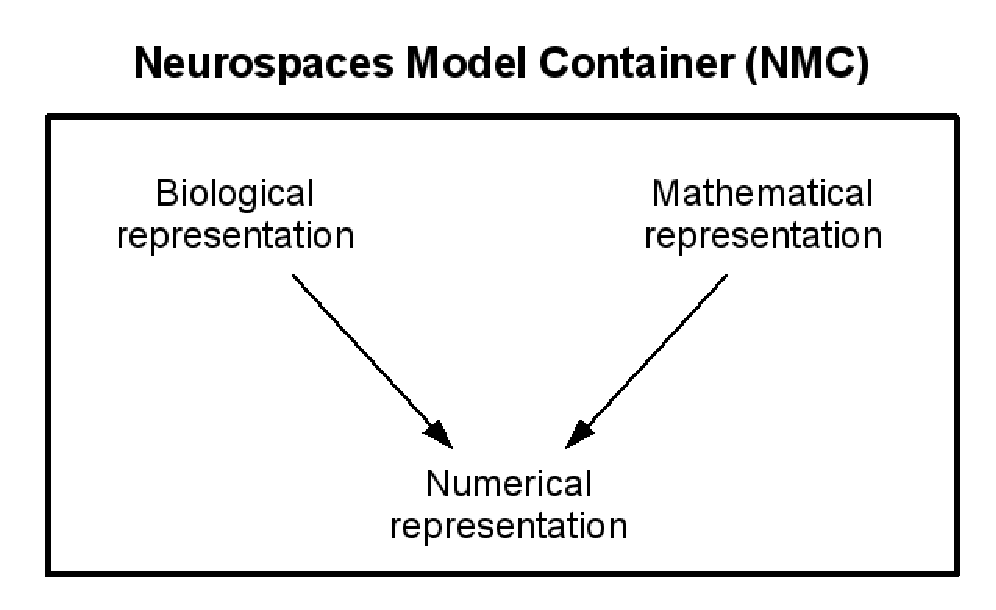
\includegraphics{figures/conversions.eps}
%  
\includegraphics[scale=0.2]{figures/matrix.png}
  \caption{NMC conversions.}
  \label{fig:nmc-conversions}
\end{figure}

For example, HH-gates are mathematical constructs based on biological
channels, such that the parameter values that define a gate are
identical to their numerical representation.

However, dendritic segments are biological constructs with a number of
mathematical properties.  They have parameters with biological values
as commonly reported in scientific papers, and must be converted to
discrete compartments and their parameters with numerical values
required for a numerical solver.  This functionality is transparant to
the user, and is explained in more detail in
sections~\ref{sec:defining-channels} and~\ref{sec:defining-soma}.


%From a user perspective, the NMC does not make a distinction between
%biological and mathematical representations of a model.  



In the next paragraphs we outline the steps required to construct an
NDF file that generates a single compartment model neuron.  This model
will be able to generate action potentials via activation of the
classical fast sodium and delayed rectifying potassium conductances as
described by Hodgkin and Huxley (HH-{\it J. Physiol.} {\bf 117}: 500).

The NDF files that generate this model can be found in the model
library at\\ {\tt /usr/local/neurospaces/models/library}. This library
is bundled with the NMC
\footnote{After installation, the channel descriptions can be found in the directory\\
  `/usr/local/neurospaces/models/library/channels/hodgkin-huxley/',\\
  while the soma model definition can be found at\\
  `/usr/local/neurospaces/models/library/segments/hodgkin\_huxley.ndf'\\
  and the neuron model definition at\\
  '/usr/local/neurospaces/models/library/tests/cells/hh1.ndf'.}.

Following installation of the NS packages you should create a working
directory for storing files used during model development (e.g. {\tt
  mkdir $\sim$/NS/HH1}).  Example commands, indicated below by \$,
were all issued after {\tt cd} to that directory.

\subsection{The HH Gates}
The HH formalism is given by sodium and potassium conductances, where
the total HH current is given by:

\begin{equation}
  \label{eq:hodgkin-huxley-current}
  I_{\mathrm{HH}} = g_{\mathrm{Na}} (V-E_{\mathrm{Na}})
  + g_{\mathrm{K}} (V-E_{\mathrm{K}}) +
  g_{\mathrm{L}}(V-E_{\mathrm{L}})
\end{equation}

where

\begin{equation}
  \label{eq:g-na}
  g_{\mathrm{Na}} = \overline{g}_{\mathrm{Na}}m^3h
\end{equation}

\begin{equation}
  \label{eq:g-k}
  g_{\mathrm{K}} = \overline{g}_{\mathrm{K}}n^4
\end{equation}

The behavior of the sodium conductance is determined by the kinetics
of the 'm' and 'h' gates, and the behavior of the potassium
conductance is determined by the kinetics of the 'n' gate.  A gate can
be in a permissive or non-permissive state, and an equation defines
the gate kinetics as transitions between those two states.  The state
of the gate is the fraction of the population of potassium channels in
a permissive state.  It assumes a value between 0 and 1.

In a NDF file a gate is defined using the \texttt{HH\_GATE} keyword.
Inside a \texttt{HH\_GATE}, the \texttt{GATE\_KINETIC\_FORWARD}
defines the parameters for transition from non-permissive to
permissive states.  The \texttt{GATE\_KINETIC\_BACKWARD} defines the
parameters for the reverse transition.

Since different simulators use different representations of the HH
formalism, the formalism used by the NMC is a generalization of the HH
formalism.  For the sake of completeness we discuss these different
representations, to define the relationship with the representation
used by the NMC.

Commonly reported in the literature are steady state and time constant
values, that are found using the formulae:

\begin{equation}
  n_\infty(V) = \frac{ \alpha_n(V) }{ \alpha_n(V) + \beta_n(V) }
\end{equation}
\begin{equation}
  \tau_n(V) = \frac{ 1 }{ \alpha_n(V) + \beta_n(V) }
\end{equation}

And relate back to $\alpha$ and $\beta$ with the following equations:

\begin{equation}
  \alpha_n(V) = \frac{ n_\infty(V) }{ \tau_n(V) }
\end{equation}
\begin{equation}
  \beta_n(V) = \frac{ 1 - n_\infty(V) }{ \tau_n(V) }
\end{equation}

For gate kinetics specification, the NMC uses an $A$-$B$ based
representation, that defines the following two functions:

\begin{equation}
  A(V) = \alpha(V)
\end{equation}
\begin{equation}
  B(V) = \frac{ 1 }{ \tau_n(V) } = \alpha(V) + \beta(V)
\end{equation}

and for converting back to the $\alpha$-$\beta$ form:

\begin{equation}
  \beta(V) = B(V) - A(V)
\end{equation}
\begin{equation}
  \alpha(V) = A(V)
\end{equation}\marginpar{give out the relationship between these
  parameters and exponential, sigmoid, linoid in the genesis sense,
  see hh\_channel docs.}

%The NMC supports the representation of the several different gate
%descriptions reported in the literature.

\paragraph{The NMC Gate Description}
The parameter names used to define a HH-like gate are based on the
above $A$-$B$ representation (a representation also used by the
GENESIS 2 {\tt tabchan} object).  Its general form is:

\begin{equation}
  \label{eq:hh-general-1}
  A(V), B(V) = \mathrm{HH\_AB\_Scale} * \frac{ ( \mathrm{HH\_AB\_Mult} * V - \mathrm{HH\_AB\_Offset\_M} ) }{ \mathrm{HH\_AB\_Add} + e ^ {\frac{ V - \mathrm{HH\_AB\_Offset\_E} }{ \mathrm{HH\_AB\_Tau} } } }
\end{equation}

In the NMC all these parameter names are prefixed with {\tt HH\_},
followed by a descriptor for the type of the gate representation, for
example {\tt AB\_} for parameters of the $A$-$B$ based representation.
In most channel descriptions the {\tt HH\_AB\_Offset\_M} parameter has a
value of zero, such that the only offset that needs to be specified is
{\tt HH\_AB\_Offset\_E}.

\begin{itemize}
\item {\tt HH\_AB\_Add}:\marginpar{Add units to all pars}.
\item {\tt HH\_AB\_Mult}:
\item {\tt HH\_AB\_Offset\_E}:
\item {\tt HH\_AB\_Offset\_M}: In most cases, {\tt HH\_AB\_Offset\_M} will be 0
  and may be omitted\marginpar{still more checks required, not
    correct}.
\item {\tt HH\_AB\_Scale}:
\item {\tt HH\_AB\_Tau}:
\end{itemize}

A last parameter is the {\tt HH\_AB\_Factor\_Flag} parameter.  It
indicates whether the exponential factor is being used as a divisor or
a multiplier:

\begin{itemize}
\item {\tt HH\_AB\_Factor\_Flag} has value -1:
\begin{equation}
  \label{eq:hh-general-ff-1}
  \mathrm{HH\_AB\_Scale} * \frac{ ( \mathrm{HH\_AB\_Mult} * V - \mathrm{HH\_AB\_Offset\_M} ) }{ \mathrm{HH\_AB\_Add} + e ^ {\frac{ V - \mathrm{HH\_AB\_Offset\_E} }{ \mathrm{HH\_AB\_Tau} } } }
\end{equation}
%\item {\tt HH\_AB\_Factor\_Flag} has value 0:
%\begin{equation}
%  \label{eq:hh-general-ff0}
%  \mathrm{HH\_AB\_Scale} * \frac{ ( \mathrm{HH\_AB\_Mult} * V - \mathrm{HH\_AB\_Offset\_M} ) }{ \mathrm{HH\_AB\_Add} + e ^ {\frac{ V - \mathrm{HH\_AB\_Offset\_E} }{ \mathrm{HH\_AB\_Tau} } } }
%\end{equation}
\item {\tt HH\_AB\_Factor\_Flag} has value 1:
\begin{equation}
  \label{eq:hh-general-ff1}
  \mathrm{HH\_AB\_Scale} * \mathrm{HH\_AB\_Add} + e ^ {\frac{ V - \mathrm{HH\_AB\_Offset\_E} }{ \mathrm{HH\_AB\_Tau} } }
\end{equation}
\end{itemize}


%\subsubsection{$\alpha$-$\beta$ based Description}
%The parameters associated with the $\alpha$-$\beta$ form
%are\footnote{It is currently not possible to define a gate using the
%  $\alpha$-$\beta$ form, or using the steady-state and tua form.}:
%\begin{itemize}
%\item {\tt Multiplier}
%\end{itemize}

%\subsubsection{Steady-state and Tau based Description}
%The parameters associated with the steady-state and tau form are:
%\begin{itemize}
%\item {\tt Multiplier}
%\end{itemize}

\subsection{Simple Parameter Specification}
\label{sec:param-spec}

For sake of brevity, we discuss the definition of the 'n' or
activation gate\marginpar{complete explanation about activation,
  inactivation deactivation, deinactivation}, and list the full
definition of all the gates.  Then, we show how to use these gate
definitions in the definition of a channel.

%$\overline{g}_{\mathrm{Na}} = 0.120$, 

The HH formalism for the potassium channel assumes a sequence of four
identical activation gates.  In
equation~(\ref{eq:g-k}) the gate state of the
potassium conductance is raised to the power of four.

The kinetics of the individual 'n' gates of the potassium channel are
determined by the functions $\alpha_h(V)$ and $\beta_h(V)$ for which
the definitions are:

\begin{equation}
  \label{eq:hh-alpha}
  \alpha_h(V) = \frac{0.01(-V + 10)}{e^{\frac{-V + 10}{10}} -
    1}
\end{equation}

\begin{equation}
  \label{eq:hh-beta}
  \beta_h(V) = 0.125 e^{ \frac{- V}{80} }
\end{equation}

In the NMC, parameters are (name, value) tuples.  Names are simple
labels.  Parameter values are defined using the {\tt PARAMETER} token,
which must occur inside a {\tt PARAMETERS} token.

In an NDF file these parameter names and values must be within the
scope of a {\tt PARAMETER} token.  For example, to set {\tt HH\_AB\_Scale}
to -600.0 in the NDF file:

\begin{verbatim}
        PARAMETER ( HH_AB_Scale = -600.0 ),
\end{verbatim}

The model parameters of the forward rate of the 'n' gate must be
grouped together by using the {\tt PARAMETERS} token.  For example:

\begin{verbatim}
      PARAMETERS
        PARAMETER ( HH_AB_Scale = -600.0 ),
        PARAMETER ( HH_AB_Mult = 10000 ),
        PARAMETER ( HH_AB_Factor_Flag = -1.0 ),
        PARAMETER ( HH_AB_Add = -1.0 ),
        PARAMETER ( HH_AB_Offset2 = 60e-3 ),
        PARAMETER ( HH_AB_Tau = -10.0e-3 ),
      END PARAMETERS
\end{verbatim}

In the same way that the NMC recognizes public and private models, the
NMC distinguishes between shared and private parameters of a model.
Because some variables are shared between model components, they must
be specifically declared, whereas this is not the case for private
parameters.

Shared variables are declared within the component they are attached
to by the {\tt INPUT} and {\tt OUTPUT} tokens, which must occur within
a block of {\tt BINDABLES}.  This allows shared variables of one
component to be bound to those of another. The binding of variables is
done with {\tt INPUT} tokens within a block of {\tt BINDINGS}.  For
example to declare {\tt Vm} as an input to the 'n' gate, and {\tt
  rate} as an output of 'n' gate:

\begin{verbatim}
    ...
      BINDABLES
        INPUT Vm, OUTPUT rate
      END BINDABLES
    ...
\end{verbatim}

To bind the {\tt Vm} of the 'n' gate to the {\tt Vm} of the parent
component, you write:

\begin{verbatim}
    ...
      BINDINGS
        INPUT ..->Vm
      END BINDINGS
    ...
\end{verbatim}

Collecting all these elements with a {\tt GATE\_KINETIC\_FORWARD}
token, the full definition of the forward rate becomes:

\begin{verbatim}
    ...
    GATE_KINETIC_A k_a
      BINDABLES
        INPUT Vm, OUTPUT rate
      END BINDABLES
      BINDINGS
        INPUT ..->Vm
      END BINDINGS
      PARAMETERS
        PARAMETER ( HH_AB_Scale = -600.0 ),
        PARAMETER ( HH_AB_Mult = 10000 ),
        PARAMETER ( HH_AB_Factor_Flag = -1.0 ),
        PARAMETER ( HH_AB_Add = -1.0 ),
        PARAMETER ( HH_AB_Offset2 = 60e-3 ),
        PARAMETER ( HH_AB_Tau = -10.0e-3 ),
      END PARAMETERS
    END GATE_KINETIC_A
    ...
\end{verbatim}

Similarly, for the backward rate we have:

\begin{verbatim}
    ...
    GATE_KINETIC_B k_b
      BINDABLES
        INPUT Vm, OUTPUT rate
      END BINDABLES
      BINDINGS
        INPUT ..->Vm
      END BINDINGS
      PARAMETERS
        PARAMETER ( HH_AB_Scale = 125.0 ),
        PARAMETER ( HH_AB_Mult = 0.0 ),
        PARAMETER ( HH_AB_Factor_Flag = -1.0 ),
        PARAMETER ( HH_AB_Add = 0.0 ),
        PARAMETER ( HH_AB_Offset2 = 70e-3 ),
        PARAMETER ( HH_AB_Tau = 80e-3 ),
      END PARAMETERS
    END GATE_KINETIC_B
    ...
\end{verbatim}


The final two parameters required for complete specification of the
'n' gate of the potassium channel, are {\tt POWER}, indicating the
power of the activation variable 'n', and {\tt state\_init}, giving
the initial state of the gate.  The reason why the initial state must
be defined is because it is a solved variable\footnote{All parameter
  names suffixed with {\tt \_init} define the initial state of a
  solved variable.}.  In GENESIS 2 the value of this parameter is
implicitly set to the steady state value of the gate at the resting
membrane potential.  This approach is good for gates with small time
constants.  However, a more general approach is to initialize the
state of the gates with values obtained after running the model (for
more information about model initialization, see also
section~\ref{model-initialization}\marginpar{explains a general way
  how to obtain initial values.}).

\begin{verbatim}
   PARAMETERS
      //m initial value, commonly forward over backward steady states
      PARAMETER ( state_init = 0.3176769097 ),
      PARAMETER ( POWER = 4.0 ),
   END PARAMETERS
\end{verbatim}


The {\tt HH\_GATE} token is used to combine the forward and backward
rate definitions, which is typically put in the public model section
of an NDF file, see figure~\ref{fig:n-gate}.

\begin{figure}[h]
  \centering
\begin{verbatim}
#!/usr/local/bin/neurospacesparse
// -*- NEUROSPACES -*-
//
// The 'n' gate specification of the HH potassium channel
//
NEUROSPACES NDF
PUBLIC_MODELS
  HH_AB_GATE k_gate_activation
    BINDABLES
      INPUT Vm,OUTPUT activation
    END BINDABLES
    BINDINGS
      INPUT ..->Vm
    END BINDINGS
    GATE_KINETIC_A k_a
      BINDABLES
        INPUT Vm, OUTPUT rate
      END BINDABLES
      BINDINGS
        INPUT ..->Vm
      END BINDINGS
      PARAMETERS
        PARAMETER ( HH_AB_Scale = -600.0 ),
        PARAMETER ( HH_AB_Mult = 10000 ),
        PARAMETER ( HH_AB_Factor_Flag = -1.0 ),
        PARAMETER ( HH_AB_Add = -1.0 ),
        PARAMETER ( HH_AB_Offset2 = 60e-3 ),
        PARAMETER ( HH_AB_Tau = -10.0e-3 ),
      END PARAMETERS
    END GATE_KINETIC_A
    GATE_KINETIC_B k_b
      BINDABLES
        INPUT Vm, OUTPUT rate
      END BINDABLES
      BINDINGS
        INPUT ..->Vm
      END BINDINGS
      PARAMETERS
        PARAMETER ( HH_AB_Scale = 125.0 ),
        PARAMETER ( HH_AB_Mult = 0.0 ),
        PARAMETER ( HH_AB_Factor_Flag = -1.0 ),
        PARAMETER ( HH_AB_Add = 0.0 ),
        PARAMETER ( HH_AB_Offset2 = 70e-3 ),
        PARAMETER ( HH_AB_Tau = 80e-3 ),
      END PARAMETERS
    END GATE_KINETIC_B
    PARAMETERS
      //m initial value, commonly forward over backward steady states
      PARAMETER ( state_init = 0.3176769097 ),
      PARAMETER ( POWER = 4.0 ),
    END PARAMETERS
  END HH_AB_GATE
END PUBLIC_MODELS
\end{verbatim}
  \caption{The 'n' gate specification of the HH potassium channel}
\label{fig:n-gate}
\end{figure}
%\afterpage{\clearpage}

As already explained, an important feature of NS is that model cells
can be constructed from a hierachy of fundamental building blocks or
library files.  The 'n' gate that we have just defined is such a
building block (see figure~\ref{fig:n-gate}).  It is being defined as
a public model in the NDF file, such that it is available to other NDF
files for use in a channel definition.  We choose to name the NDF file
{\tt k\_gate.ndf}.  The channel definition is then available for
incorporation into the model soma (described in
section~\ref{sec:defining-soma}).

For a more complete description of parameter and function
specifications, see the multi-compartmental section
(section~\ref{sec:multi-comp}).

%  Functions can have regular parameters.
%For example, the Nernst equation description of the control of the
%potassium reversal potential by the intracellular calcium
%concentration:

%\begin{verbatim}
%PARAMETERS
%   PARAMETER ( Ek = NERNST
%               (PARAMETER ( Cin = ../Ca_pool->conc ),
%                PARAMETER ( Cout = 2.4 ),
%                PARAMETER ( valency = ../Ca_pool->VAL ), /* 2+ */
%                PARAMETER ( T = 37.0 ))
%END PARAMETERS
%\end{verbatim}

%The definition of a model is always associated with a {\tt BINDABLES}
%specification, while the use of a {\tt CHILD} token is always
%associated with a {\tt BINDINGS} specification.

\subsection{Defining Channels}
\label{sec:defining-channels}
Every channel model consists of a number of gates.  We have shown in
the previous section how to define a single gate model based on the
HH $A$-$B$ formalism.  This gate model was given the name {\tt
  k\_gate\_activation}, and placed in the public model section of a
NDF file with the name {\tt k\_gate.ndf}.  It is then availabe for use
in other model files.

To use the gate model, the public model section is imported with a
{\tt FILE} token and assigned to a namespace, here {\tt k\_gate}.
% (see
%figure~\ref{fig:n-gate-import}).
The {\tt ALIAS} token, {\tt HH\_K\_n}, makes the gate model available
to the public models of the importing file:
%  The gate model is then made available to the
%public models of the importing file under the name {\tt HH\_K\_n} by
%using the {\tt ALIAS} token 

%\begin{figure}[h]
\begin{center}
%  \begin{boxedminipage}{13cm}
\begin{verbatim}
#!/usr/local/bin/neurospacesparse
// -*- NEUROSPACES -*-
//
// Importing and inserting the 'n' gate specification
// of the HH potassium channel
//
NEUROSPACES NDF
IMPORT
    FILE k_gate "k_gate.ndf"
END IMPORT
PRIVATE_MODELS
    ALIAS k_gate::/k_gate_activation HH_K_n END ALIAS
END PRIVATE_MODELS
...
\end{verbatim}
\end{center}
%  \end{boxedminipage}

After definition of the 'n' gate, the potassium channel can be defined
using the parameters {\tt G\_MAX}, {\tt E\_REV}, and {\tt
  CHANNEL\_TYPE}.  {\tt G\_MAX} and {\tt E\_REV} define the
conductance density and the channel reversal potential, respectively
(see equation~(\ref{eq:hodgkin-huxley-current}),
page~\pageref{eq:hodgkin-huxley-current}).  The third parameter, {\tt
  CHANNEL\_TYPE}, distinguishes between channels with activation gates
only (value {\tt ``ChannelAct''}), and channels with both activation
and inactivation gates (value {\tt ``ChannelActInact''}).  The {\tt
  CHILD} token links the gate with the channel model:
%  This is
%shown in figure~\ref{fig:n-gate-import}.

\begin{center}
%  \begin{boxedminipage}{13cm}
\begin{verbatim}
...
PUBLIC_MODELS
    CHANNEL k
        BINDABLES
            INPUT Vm,OUTPUT G,OUTPUT I
        END BINDABLES
        PARAMETERS
            PARAMETER ( CHANNEL_TYPE = "ChannelAct" ),
        END PARAMETERS
        CHILD HH_K_n n
        END CHILD
        PARAMETERS
            PARAMETER ( G_MAX = 360.0 ),
            PARAMETER ( E_REV = -0.082 ),
        END PARAMETERS
    END CHANNEL
END PUBLIC_MODELS
\end{verbatim}
%  \end{boxedminipage}
\end{center}
%  \caption{Top panel: Importing the 'n' gate specification of the HH
%    potassium channel into a new NDF file.  Bottom panel: Inserting
%    the 'n' gate specification into the HH potassium channel}
%\label{fig:n-gate-import}
%\end{figure}
%\afterpage{\clearpage}


%\begin{figure}[h]
%  \centering
%  \caption{Inserting the 'n' gate specification of the HH potassium
%    channel}
%\label{fig:n-gate-insert}
%\end{figure}
%\afterpage{\clearpage}

\subsection{Defining the Soma}
\label{sec:defining-soma}

Historically, neuronal somas have been modeled as cylinders, but
visualized as spheres.  The NMC supports both specifications.  A
spherical representation is given by the {\tt SPHERICAL} option, and
the {\tt DIA} parameter defines the diameter of the sphere.  For
expediency, the spherical representation is converted to its
cylindrical equivalent for numerical computation\footnote{Such
  conversion was also implemented by the GENESIS 2 simulator.}.  It
has membrane properties, for which we have to specify the appropriate
parameters: specific resistance {\tt RM}, specific capacitance {\tt
  CM} and the reversal potential for the leak conductance {\tt ELEAK}.

\begin{equation}
  \label{eq:cable-no-space}
  \mathrm{C_m} \frac{dVm}{dt} + \frac{Vm - \mathrm{ELEAK}}{\mathrm{R_m}} + I_{\mathrm{HH}} = 0
\end{equation}

where $I_{\mathrm{HH}}$ is defined by
equation~(\ref{eq:hodgkin-huxley-current}), and

\begin{equation}
  \label{eq:cable-no-space-cm}
  \mathrm{C_m} = \mathrm{CM} \, 4 \pi \left( \frac{\mathrm{DIA}}{2} \right) ^2 = \pi \, \mathrm{CM} \, (\mathrm{DIA}) ^2
\end{equation}

\begin{equation}
  \label{eq:cable-no-space-rm}
  \mathrm{R_m} = \frac{\mathrm{RM}}{4 \pi \left( \frac{\mathrm{DIA}}{2} \right) ^2} = \frac{\mathrm{RM}}{\pi \, (\mathrm{DIA}) ^2}
\end{equation}

%For the cylindrical representation, see section~\ref{sec:multi-comp}.

Just as the initial state of the gates was defined (see
section~\ref{sec:param-spec}), the initial state of the cell membrane
must be defined, here using the {\tt Vm\_init} parameter.
%This is
%given in figure~\ref{fig:soma}.

%            PARAMETER ( RA = 0.3 ),
%\begin{figure}[h]
\begin{center}
%  \begin{boxedminipage}{13cm}
\begin{verbatim}
    SEGMENT soma
        ...
        OPTIONS SPHERICAL
        PARAMETERS
            PARAMETER ( Vm_init = -0.07 ),
            PARAMETER ( RM = 0.33333 ),
            PARAMETER ( CM = 0.01 ),
            PARAMETER ( ELEAK = -0.0594 ),
            PARAMETER ( DIA = 30e-6 ),
        END PARAMETERS
        ...
    END SEGMENT
\end{verbatim}
%  \end{boxedminipage}
%  \caption{Soma parameter definitions}
%\label{fig:soma}
%\end{figure}
\end{center}

To insert the previously defined sodium and potassium channel models
into the membrane, they are assigned as children of the soma segment.
The channels provide a current that forms the input to the segment
($I_\mathrm{HH}$, see equation~(\ref{eq:cable-no-space}).  The segment
gives rise to the membrane potential, which is passed to the channels.
The relationship between a channel and the membrane is formed by using
shared variables that are declared using the {\tt BINDABLES} token.
The binding of the shared variables is done with {\tt INPUT} tokens
within a block of {\tt BINDINGS} (see also
section~\ref{sec:param-spec}):
% (see
%figure~\ref{fig:soma-channel}).

%\begin{figure}[h]
\begin{center}
%    \begin{boxedminipage}{13cm}
\begin{verbatim}
    ...
    SEGMENT soma
        BINDABLES
            OUTPUT Vm
        END BINDABLES
        BINDINGS
            INPUT k->I,
            INPUT na->I,
        END BINDINGS
        OPTIONS SPHERICAL
        PARAMETERS
            PARAMETER ( Vm_init = -0.07 ),
            PARAMETER ( RM = 0.33333 ),
            PARAMETER ( RA = 0.3 ),
            PARAMETER ( CM = 0.01 ),
            PARAMETER ( ELEAK = -0.0594 )
            PARAMETER ( DIA = 30e-6 ),
        END PARAMETERS
        CHILD na na
            BINDINGS
                INPUT ^->Vm
            END BINDINGS
        END CHILD
        CHILD k k
            BINDINGS
                INPUT ^->Vm
            END BINDINGS
        END CHILD
    END SEGMENT
    ...
\end{verbatim}
\end{center}
%  \end{boxedminipage}
%  \caption{Soma with sodium and potassium HH-channels}
%\label{fig:soma-channel}
%\end{figure}

The complete NDF file with the definition of the soma is shown in
figure~\ref{fig:soma-channels-complete}.

\begin{figure}[h]
  \centering
%  \begin{boxedminipage}{13cm}
\begin{verbatim}
#!neurospacesparse
// -*- NEUROSPACES -*-
NEUROSPACES NDF
IMPORT
    FILE k "channels/hodgkin-huxley/potassium.ndf"
    FILE na "channels/hodgkin-huxley/sodium.ndf"
END IMPORT
PRIVATE_MODELS
    ALIAS k::/k k END ALIAS
    ALIAS na::/na na END ALIAS
    SEGMENT soma
        BINDABLES
            OUTPUT Vm
        END BINDABLES
        BINDINGS
            INPUT k->I,
            INPUT na->I,
        END BINDINGS
        OPTIONS SPHERICAL
        PARAMETERS
            PARAMETER ( Vm_init = -0.07 ),
            PARAMETER ( RM = 0.33333 ),
            PARAMETER ( RA = 0.3 ),
            PARAMETER ( CM = 0.01 ),
            PARAMETER ( ELEAK = -0.0594 )
            PARAMETER ( DIA = 30e-6 ),
        END PARAMETERS
        CHILD na
            na
            BINDINGS
                INPUT ^->Vm
            END BINDINGS
        END CHILD
        CHILD k
            k
            BINDINGS
                INPUT ^->Vm
            END BINDINGS
        END CHILD
    END SEGMENT
END PRIVATE_MODELS
PUBLIC_MODELS
    ALIAS soma hh_segment END ALIAS
END PUBLIC_MODELS
\end{verbatim}
%  \end{boxedminipage}
  \caption{Soma parameter definitions}
\label{fig:soma-channels-complete}
\end{figure}
%\afterpage{\clearpage}


\subsection{The Neuron Model}
\label{sec:neuron-model}
To complete the neuron model, the soma must be inserted into the model
cell.  This is done by importing the soma definition into the private
model section of a NDF file.  The {\tt ALIAS} token makes the
definition available to the public model section (see also
section~\ref{sec:defining-channels}).  The model cell is then created
using a {\tt CELL} token, and the soma segment is assigned as a child
inside this token:

\begin{center}
\begin{verbatim}
#!/usr/local/bin/neurospacesparse
// -*- NEUROSPACES -*-
//
// Importing and inserting a soma into a cell.
//
NEUROSPACES NDF
IMPORT
    FILE soma "hh_soma.ndf"
END IMPORT
PRIVATE_MODELS
    ALIAS soma::/hh_segment hh_segment END ALIAS
END PRIVATE_MODELS
PUBLIC_MODELS
    CELL hh_neuron
        SEGMENT_GROUP segments
            CHILD hh_segment soma END CHILD
        END SEGMENT_GROUP
    END CELL
END PUBLIC_MODELS
\end{verbatim}
\end{center}


\subsection{Running a Simulation}
\label{sec:running-simulation}
A simulation is started using the {\tt ssp} command.  This reads a SSP
configuration file that controls the simulation, including the
stimulation protocol and simulation output.  For expediency, the {\tt
  ssp} command has builtin configurations for running different types
of simulation\footnote{For more information about the builtin
  configuration, use '{\tt ssp --builtins}'.}.  The '{\tt --cell}'
option selects the builtin configuration for running a single neuron
model.  The required argument is a reference to the NDF file that
contains the model to be simulated.  First, an environment variable is
set to instruct the NMC where to find this file:

{\tt \$ export
  NEUROSPACES\_NMC\_USER\_MODELS=/usr/local/neurospaces/models/library/examples}

Then, we can run the model:

{\tt \$ ssp --cell hh\_neuron.ndf}

The duration of the simulation and its temporal resolution are given
respectively by the {\tt --time} and {\tt --time-step} options.  Both
options take an amount of time specified in seconds.  The default time
step is 20$\,\mu$s (2e-5$\,$s in SI units), while the default
simulation time is 50$\,$ms.
%  The {\tt --steps} is an
%alternative way to define the simulation time.

{\tt \$ ssp --cell hh\_neuron.ndf --time 0.5}

By default, the output of a simulation using the {\tt --cell}
configuration is the membrane potential at the soma.  It is stored in
a file that takes its name from the NDF argument passed to SSP.  For
our single compartment model, this is {\tt output/hh\_neuron}.
Additional command line options are available that overwrite specific
{\tt --cell} defaults, and define other stimuli and outputs.  For
example, the {\tt --inject-magnitude} option specifies the magnitude
of somatic current injection.  The time course of the current
injection is given by the {\tt --inject-delay} and {\tt
  --inject-duration} options.  The {\tt --parameters} option will
allow initialization of other input parameters.

For example to inject a current into the soma with magnitude 2$\,$nA
for the duration of the simulation:

{\tt \$ ssp --cell hh\_neuron.ndf --time 0.5 --inject 2e-9}

To run the same simulation using the {\tt parameters} option:

{\tt \$ ssp --cell hh\_neuron.ndf --time 0.5 --parameter
  '/cell/soma->INJECT=1e-9'}

Here, the {\tt --parameters} option assigns a value to a model
parameter using a syntax specific for the NMC.  Note that the use of
single quotes is required to protect the argument string from being
interpreted as an output redirection command to a file with a peculiar
name.

Specific outputs are defined with the {\tt --output} option.  The
default filename for this option is inferred from the NDF filename,
and this file is placed in the directory {\tt ./output/}, which is
created if it does not exist.  For example, to store the somatic
membrane potential, the command:

{\tt \$ ssp --cell hh\_neuron.ndf --time 0.5 --parameter
  '/cell/soma->INJECT=1e-9' --output '/cell/soma->Vm'}

will generate an output file named {\tt output/hh\_neuron.out}.  By
convention, the default output filename has an {\tt .out} extension.
The output filename can be changed using the {\tt
  --outputclass-filename} option\marginpar{implement}.

{\tt \$ ssp --cell hh\_neuron.ndf --time 0.5 --parameter
  '/cell/soma->INJECT=1e-9' --output '/cell/soma->Vm'
  --outputclass-filename hh\_neuron/inject1e-9.out}

Note that the {\tt ./hh\_neuron/} directory is also created
automatically.


\paragraph{Synaptic stimulation}

The model defined in the previous sections does not contain synapses,
and can only be stimulated by current injection.  Here, we first show
how to add synapses to the model, and then how to activate the them.

Synaptic activation can be done in two ways: the first method of
activation is to set the firing frequency of spontaneous activity.
This frequency is a parameter of the synaptic channel, and the weight
of the activated synapse is always one.  This type of activation is
commonly used to simulated an in-vivo condition.

The second method of activation is given by attaching a series of
precalculated synaptic event times stored in a file to the synaptic
channel.

{\tt \$ ssp --cell hh\_neuron.ndf --parameter
  '/cell/soma/afferent[0]->INJECT=1e-9'}\marginpar{add afferents to
  the model}




% \begin{center}
% \begin{verbatim}
%\$ ssp --builtins
%/usr/local/bin/ssp <configuration>
%/usr/local/bin/ssp: run simulations, given an ssp configuration, or using a builtin configuration

%Known builtin configurations:

%cell:

%        Simulate a single model neuron, default is to output the membrane potential of the soma.
%        Use the options to inject current in the soma (--inject).
%        The model's soma segment must reside in a SEGMENT_GROUP with name "segments".

%        The name of the model neuron is inferred from the name of the model description file.
%        (e.g. a model description file called "hh_neuron.ndf" is assumed to define a model neuron
%        called "hh_neuron").

%        --model-name overwrite the default model name.
%        --steps sets number of steps
% \end{verbatim}
% \end{center}

When using builtin configurations, the names of the simulation
schedule and the output file can be defined using the command line
flags {\tt --set-name} and {\tt --set-outputclass-filename},
respectively.


\subsection{Initialization of Simulation Variables}

\begin{itemize}
\item {\tt --dump-variables}
\item {\tt --undump-variables}
\end{itemize}


\section{A Multicompartmental Model}
\label{sec:multi-comp}

\subsection{Morphology}

Discuss morphology2ndf overhere.

\subsection{Symbolic Parameter Specifications}

%The HH formalism for the potassium channel assumes a sequence of four
%identical activation gates.  In
%equation~(\ref{eq:hodgkin-huxley-current}) the gate state of the
%potassium conductance is raised to the power of four.  This is given
%by the {\tt POWER} parameter value in this example.
% Values are either constant, point to a parameter of another symbol,
% or have a function value.  As an example:
%\begin{verbatim}
%PARAMETERS
%   PARAMETER ( DIAMETER = 0.3 ),
%   PARAMETER ( LENGTH = ..->LENGTH ),
%   PARAMETER ( SEED = SERIAL () )
%END PARAMETERS
%\end{verbatim}
% Here, the {\tt DIAMETER} parameter has a constant value, the {\tt
%   LENGTH} parameter is inherited from the parent component (the
% '$..$' notation is a reference to the parent symbol\footnote{The NDF
%   format supports both the '$..$', and $^\wedge$ notations to
%   reference the parent symbol.  While non-technical people might
%   prefer the $^\wedge$ notation, an informal survey suggests that
%   technical people will prefer the '$..$' notation.}), and {\tt
%   SEED} has a value defined by the function {\tt SERIAL()}.

\subsection{Running the model}


\section{The Morphology Convertor}
\label{sec:morph-conv-conf}

A {\tt .ndf} file can be generated from a {\tt
  .swc} (or a GENESIS {\tt .p}) morphology file by running:

\vspace{2mm}

{\tt \$ morphology2ndf <directorypath>/fname.swc >
  <directorypath>/fname.ndf}

\vspace{2mm}

Note the redirection arrow ($>$) in the above statement. A list of the
optional conversion parameters is obtained with:

\vspace{2mm}

{\tt \$ morphology2ndf -h}

\vspace{2mm}

As mentioned above, neuron morphology files can be converted to NDF
files using the command {\tt morphology2ndf}.  Under normal
circumstances this command is called and configured automatically by
the simulator.  The configuration of this command is done via a
configuration file.  If a configuration file is not given as a flagged
argument in the command line (e.g. {\tt morphology2ndf fname.swc
  --configuration fname.config}) a default configuration file based on
the De Schutter \& Bower 1994 Purkinje neuron paper ({\it J.
  Neurophysiol.} {\bf 71}: 375) is used. The contents of this file
(which is currently being used by regression tests) is obtained with:

\vspace{2mm}

{\tt \$ morphology2ndf --show-config}

\vspace{2mm}

which returns:

\begin{verbatim}
---
options:
  histology:
    shrinkage: 1                                     // Multiplicative shrinkage correction factor
  relocation:
    soma_offset: 1                                   // Boolean flag signalling relocation of origin
prototypes:
  aliasses:                                          // Files declaring characteristics of each morphological element
    - segments/spines/purkinje.ndf::Purk_spine
    - tests/segments/purkinje/maind.ndf::maind
    - tests/segments/purkinje/soma.ndf::soma
    - tests/segments/purkinje/spinyd.ndf::spinyd
    - tests/segments/purkinje/thickd.ndf::thickd
  parameter_2_prototype:                             // Given dendritic diameters partition morphological elements
    - dia: 3.18e-06
      prototype: spinyd
    - dia: 7.71e-06
      prototype: thickd
    - dia: 2.8e-05
      prototype: maind
    - dia: 1
      prototype: soma
  spine_prototypes: []
variables:
  origin:
    x: 0
    y: 0
    z: 0
\end{verbatim}

%---
%library: {}
%options:
%   histology:
%      shrinkage: 1
%   relocation:
%      soma_offset: 1
%prototypes:
%   aliasses:
%      - segments/spines/purkinje.ndf::Purk_spine
%      - tests/segments/purkinje/maind.ndf::maind
%      - tests/segments/purkinje/soma.ndf::soma
%      - tests/segments/purkinje/spinyd.ndf::spinyd
%      - tests/segments/purkinje/thickd.ndf::thickd
%    name_2_prototype:
%      - name: 'br1[0]'
%        prototype: thickd
%      - name: 'br2[0]'
%        prototype: thickd
%      - name: 'b1s06[1]'
%        prototype: thickd
%      - name: 'b1s06[2]'
%        prototype: thickd
%      - name: 'b1s10[23]'
%        prototype: spinyd
%      - name: 'b2s30[10]'
%        prototype: spinyd
%      - name: 'b3s37[18]'
%        prototype: spinyd
%      - name: 'b3s44[26]'
%        prototype: spinyd
%      - name: 'b3s45[4]'
%        prototype: spinyd
%      - name: 'b3s45[12]'
%        prototype: spinyd
%      - name: 'b3s45[20]'
%        prototype: spinyd
%    parameter_2_prototype:
%      - dia: 3.18e-06
%        prototype: spinyd
%      - dia: 7.71e-06
%        prototype: thickd
%      - dia: 2.8e-05
%        prototype: maind
%      - dia: 1
%        prototype: soma
%   spine_prototypes: []
%variables:
%   origin:
%      x: 0
%      y: 0
%      z: 0

We note that in the configuration file, the value indicator
(http://www.yaml.org/refcard.html), a single colon (:), indicates an
unordered list (see in above example following {\tt aliasses}) and the
nested series indicator, a dash (-), indicates an ordered list (see in
above example following {\tt parameter\_2\_prototype}).  Importantly,
we note that the configuration file is white space sensitive and
tabulators are not allowed for spacing.

The `aliasses' of the configuration file:
\begin{verbatim}
prototypes:
  aliasses:
    - segments/motorpyramidal/py23soma.ndf::soma
    - segments/motorpyramidal/py23dend.ndf::dendrite
    - segments/motorpyramidal/py23apicaldend.ndf::apical_dendrite
    - segments/motorpyramidal/py23axon.ndf::axon
\end{verbatim}
are inserted into the scope of the IMPORT token in the NDF file during
the command:

\vspace{2mm}

{\tt \$ morphology2ndf <fname>.swc --configuration <fname.config> >
  <fname>.ndf}

\vspace{2mm}

The default entries for the key {\tt parameter\_2\_prototype}
enumerate the {\tt prototype}(s) in order of increasing diameter.
Thus, (i) spiny dendrites include all compartments $<$ 3.18e$^{-6}$,
(ii) 3.18e$^{-6} <$ thick dendrites $<$ 7.71e$^{-6}$, (iii)
7.71e$^{-6} <$ main dendrite $<$ 2.8e$^{-5}$, and (iv) 2.8e$^{-5} <$
soma $<$ 1.

An alternative way to specify prototypes in the configuration file is
with the flags defined for a .swc morphology file that tag the
location of different neuronal compartments:

\begin{verbatim}
   parameter_2_prototype: // Given .swc defined flags tag morphological elements
      - tag: 1
        prototype: soma
      - tag: 2
        prototype: axon
      - tag: 3
        prototype: dendrite
      - tag: 4
        prototype: apical_dentrite
\end{verbatim}

The De Schutter and Bower (1994) Purkinje cell model can not be
exactly reproduced this way from its original morphology file.  This
is due to a small difference between the distribution of the active
channels in the model vs. the output of {\tt morphology2ndf}.  To
solve this problem, a second key ({\tt name\_2\_prototype}) can be
optionally included into the configuration file.  It defines a mapping
of names to prototypes as opposed to parameters to prototypes. The key
behaves essentially the same as{\tt parameter\_2\_prototype}, but
instead of looking at a parameter value such as {\tt dia} or {\tt
  tag}, it looks at the names of the segments in the morphology file.
When the name matches, this key takes higher priority than the {\tt
  parameter\_2\_prototype} key.  Thus a regular mapping of the
morphology to an active model is given using the {\tt
  parameter\_2\_prototype} key with an additional number of hardcoded
exceptions given by the key {\tt name\_2\_prototype'}, such that {\tt
  morphology2ndf} can produce an exact match with the Purkinje cell
model.

Note that the inline comments included in the above examples and
indicated by {\tt //} are inserted here for clarification but are not
permitted in the actual configuration file. As mentioned above, the
command line arguments to {\tt morphology2ndf} can be used to
overwrite default configuration values before any conversion takes
place, e.g. to change the shrinkage factor:

\vspace{2mm}

{\tt \$ morphology2ndf fname.swc (or .p) --configuration fname.config
  --shrinkage 1.1111 > my.ndf}

\vspace{2mm}

This will replace the default shrinkage correction factor of 1 with
the given value (1.1111) in {\tt my.ndf}.

%Files within the scope of the IMPORT token can be unordered in the
%$<$fname$>$.config file. When the NDF file is constructed by running
%{\tt morphology2ndf} on the configuration file, the imported files are
%sorted into alphabetical order:


%\newpage

%\subsection{The NDF File Structure}
%\label{subsec:ndf-file-struct}

%An important feature of NS is that model cells can be constructed from
%a hierachy of fundamental building blocks or library files. The model
%cell that we describe here is composed of three such files that are
%called recursively from within the root file. This number of files
%results from the number of library files that are combined to build
%the example model cell. For convenience we now list the contents of
%these files.

%\subsubsection{hh1.ndf}
%This is the NDF file that combines the elements of the model into a
%single location or root file.
%\begin{verbatim}
%#!/usr/local/bin/neurospacesparse
%// -*- NEUROSPACES -*-

%NEUROSPACES NDF

%IMPORT

%   FILE hh "segments/hodgkin_huxley.ndf"

%END IMPORT

%PRIVATE_MODELS

%   ALIAS hh::/hh_segment hh END ALIAS

%END PRIVATE_MODELS

%PUBLIC_MODELS

%   CELL hh1

%      SEGMENT_GROUP segments

%         CHILD hh soma
%         END CHILD

%      END SEGMENT_GROUP

%   END CELL

%END PUBLIC_MODELS
%\end{verbatim}
%\subsubsection{hodgkin\_huxley.ndf}
%Defines the soma of the example cell.
%\begin{verbatim}
%#!/usr/local/bin/neurospacesparse
%// -*- NEUROSPACES -*-

%NEUROSPACES NDF

%IMPORT

%   FILE k "channels/hodgkin-huxley/potassium.ndf"
%   FILE na "channels/hodgkin-huxley/sodium.ndf"

%END IMPORT

%PRIVATE_MODELS

%   ALIAS k::/k k END ALIAS
%   ALIAS na::/na na END ALIAS

%   SEGMENT soma

%      BINDABLES
%         OUTPUT Vm
%      END BINDABLES

%      BINDINGS
%         INPUT k->Ik,
%         INPUT na->Ik,
%      END BINDINGS

%      OPTIONS SPHERICAL

%      PARAMETERS
%         PARAMETER ( Vm_init = -0.07 ),
%         PARAMETER ( RM = 0.33333 ),
%         PARAMETER ( RA = 0.3 ),
%         PARAMETER ( CM = 0.01 ),
%         PARAMETER ( ELEAK = -0.0594 )
%      END PARAMETERS

%      PARAMETERS
%         PARAMETER ( rel_X = 0.000e-6 ),
%         PARAMETER ( rel_Y = 0.000e-6 ),
%         PARAMETER ( rel_Z = 0.000e-6 ),
%         PARAMETER ( DIA = 30e-6 ),
%      END PARAMETERS

%      CHILD na
%         na
%         BINDINGS
%            INPUT ..->Vm
%         END BINDINGS
%      END CHILD

%      CHILD k
%         k
%         BINDINGS
%            INPUT ..->Vm
%         END BINDINGS
%      END CHILD

%   END SEGMENT


%END PRIVATE_MODELS

%PUBLIC_MODELS

%   ALIAS soma hh_segment END ALIAS

%END PUBLIC_MODELS
%\end{verbatim}
%\subsubsection{potassium.ndf}
%Defines the properties of a HH potassium conductance.
%\begin{verbatim}
%#!/usr/local/bin/neurospacesparse
%// -*- NEUROSPACES -*-

%NEUROSPACES NDF

%PRIVATE_MODELS

%   HH_AB_GATE k_gate_activation
%      BINDABLES
%         INPUT Vm,OUTPUT activation
%      END BINDABLES

%      BINDINGS
%         INPUT ..->Vm
%      END BINDINGS

%      GATE_KINETIC_FORWARD forward

%         BINDABLES
%            INPUT Vm, OUTPUT rate
%         END BINDABLES

%         BINDINGS
%            INPUT ..->Vm
%         END BINDINGS

%         PARAMETERS

%            //m 1: multiplier

%            PARAMETER ( Multiplier = -600.0 ),

%            //m 2: multiplier membrane dependence, 0.0 for no dependence

%            PARAMETER ( MembraneDependence = 10000 ),

%            //m 3: choose between nominator or denominator, 1 means nominator, -1
%            //m means denominator

%            PARAMETER ( Nominator = -1.0 ),

%            //m 4: nominator or denominator offset

%            PARAMETER ( DeNominatorOffset = -1.0 ),

%            //m 5: membrane offset

%            PARAMETER ( MembraneOffset = 60e-3 ),

%            //m 6: denormalized time constant

%            PARAMETER ( TauDenormalizer = -10.0e-3 ),

%         END PARAMETERS

%      END GATE_KINETIC_FORWARD

%      GATE_KINETIC_BACKWARD backward

%         BINDABLES
%            INPUT Vm, OUTPUT rate
%         END BINDABLES

%         BINDINGS
%            INPUT ..->Vm
%         END BINDINGS

%         PARAMETERS

%            //m 1: multiplier

%            PARAMETER ( Multiplier = 125.0 ),

%            //m 2: multiplier membrane dependence, 0.0 for no dependence

%            PARAMETER ( MembraneDependence = 0.0 ),

%            //m 3: choose between nominator or denominator, 1 means nominator, -1
%            //m means denominator

%            PARAMETER ( Nominator = -1.0 ),

%            //m 4: nominator or denominator offset

%            PARAMETER ( DeNominatorOffset = 0.0 ),

%            //m 5: membrane offset

%            PARAMETER ( MembraneOffset = 70e-3 ),

%            //m 6: denormalized time constant

%            PARAMETER ( TauDenormalizer = 80e-3 ),

%         END PARAMETERS

%      END GATE_KINETIC_BACKWARD

%      PARAMETERS

%         //m initial value, commonly forward over backward steady states

%         PARAMETER ( state_init = 0.3176769097 ),
%         PARAMETER ( POWER = 4.0 ),
%      END PARAMETERS

%   END HH_AB_GATE

%   CHANNEL k
%      BINDABLES
%         INPUT Vm,OUTPUT Gk,OUTPUT Ik
%      END BINDABLES

%      PARAMETERS
%         PARAMETER ( CHANNEL_TYPE = "ChannelAct" ),
%      END PARAMETERS

%      CHILD k_gate_activation k_gate_activation
%      END CHILD

%      PARAMETERS
%         PARAMETER ( G_MAX = 360.0 ),
%         PARAMETER ( Ek = -0.082 ),
%      END PARAMETERS
%   END CHANNEL

%   SEGMENT soma2

%      BINDABLES
%         OUTPUT Vm
%      END BINDABLES

%      BINDINGS
%         INPUT k->Ik,
%      END BINDINGS

%      OPTIONS SPHERICAL

%      PARAMETERS
%         PARAMETER ( Vm_init = -0.07 ),
%         PARAMETER ( RM = 0.33333 ),
%         PARAMETER ( RA = 0.3 ),
%         PARAMETER ( CM = 0.01 ),
%         PARAMETER ( ELEAK = -0.0594 ),
%      END PARAMETERS

%      CHILD k
%         k
%         BINDINGS
%            INPUT ..->Vm,
%         END BINDINGS
%      END CHILD

%   END SEGMENT

%END PRIVATE_MODELS

%PUBLIC_MODELS

%   // the sodium channel for import from other models

%   ALIAS k k END ALIAS

%   // a soma only test neuron with only this channel

%   CELL cell_k

%      SEGMENT_GROUP segments

%         CHILD soma2 soma
%            PARAMETERS
%               PARAMETER ( rel_X = 0.000e-6 ),
%               PARAMETER ( rel_Y = 0.000e-6 ),
%               PARAMETER ( rel_Z = 0.000e-6 ),
%               PARAMETER ( DIA = 30e-6 ),
%            END PARAMETERS
%         END CHILD

%      END SEGMENT_GROUP

%   END CELL

%   // the same neuron, yet cylindrical

%   CELL cell_k

%      SEGMENT_GROUP segments

%         CHILD soma2 soma
%            PARAMETERS
%               PARAMETER ( rel_X = 0.000e-6 ),
%               PARAMETER ( rel_Y = 0.000e-6 ),
%               PARAMETER ( rel_Z = 0.000e-6 ),
%               PARAMETER ( DIA = 30e-6 ),
%               PARAMETER ( LENGTH = 30e-6 ),
%            END PARAMETERS
%         END CHILD

%      END SEGMENT_GROUP

%   END CELL

%END PUBLIC_MODELS


%\end{verbatim}
%\subsubsection{sodium.ndf}

%Defines the properties of a HH sodium conductance.

%\begin{verbatim}
%#!/usr/local/bin/neurospacesparse
%// -*- NEUROSPACES -*-

%NEUROSPACES NDF

%PRIVATE_MODELS

%   HH_AB_GATE na_gate_activation
%      BINDABLES
%         INPUT Vm,OUTPUT activation
%      END BINDABLES

%      BINDINGS
%         INPUT ..->Vm
%      END BINDINGS

%      GATE_KINETIC_FORWARD forward

%         BINDABLES
%            INPUT Vm, OUTPUT rate
%         END BINDABLES

%         BINDINGS
%            INPUT ..->Vm
%         END BINDINGS

%         PARAMETERS

%            //m 1: multiplier

%            PARAMETER ( Multiplier = -4500.0 ),

%            //m 2: multiplier membrane dependence, 0.0 for no dependence

%            PARAMETER ( MembraneDependence = 0.1e6 ),

%            //m 3: choose between nominator or denominator, 1 means nominator, -1
%            //m means denominator

%            PARAMETER ( Nominator = -1.0 ),

%            //m 4: nominator or denominator offset

%            PARAMETER ( DeNominatorOffset = -1.0 ),

%            //m 5: membrane offset

%            PARAMETER ( MembraneOffset = 0.045 ),

%            //m 6: denormalized time constant

%            PARAMETER ( TauDenormalizer = -0.01 ),

%         END PARAMETERS

%      END GATE_KINETIC_FORWARD

%      GATE_KINETIC_BACKWARD backward

%         BINDABLES
%            INPUT Vm, OUTPUT rate
%         END BINDABLES

%         BINDINGS
%            INPUT ..->Vm
%         END BINDINGS

%         PARAMETERS

%            //m 1: multiplier

%            PARAMETER ( Multiplier = 4e3 ),

%            //m 2: multiplier membrane dependence, 0.0 for no dependence

%            PARAMETER ( MembraneDependence = 0.0 ),

%            //m 3: choose between nominator or denominator, 1 means nominator, -1
%            //m means denominator

%            PARAMETER ( Nominator = -1.0 ),

%            //m 4: nominator or denominator offset

%            PARAMETER ( DeNominatorOffset = 0.0 ),

%            //m 5: membrane offset

%            PARAMETER ( MembraneOffset = 0.07 ),

%            //m 6: denormalized time constant

%            PARAMETER ( TauDenormalizer = 18e-3 ),

%         END PARAMETERS

%      END GATE_KINETIC_BACKWARD

%      PARAMETERS

%         //m initial value, commonly forward over backward steady states

%         PARAMETER ( state_init = 0.05293248736 ),
%         PARAMETER ( POWER = 3.0 ),
%      END PARAMETERS

%   END HH_AB_GATE

%   HH_AB_GATE na_gate_inactivation
%      BINDABLES
%         INPUT Vm,OUTPUT activation
%      END BINDABLES

%      BINDINGS
%         INPUT ..->Vm
%      END BINDINGS

%      GATE_KINETIC_FORWARD forward

%         BINDABLES
%            INPUT Vm, OUTPUT rate
%         END BINDABLES

%         BINDINGS
%            INPUT ..->Vm
%         END BINDINGS

%         PARAMETERS

%            //m 1: multiplier

%            PARAMETER ( Multiplier = 70.0 ),

%            //m 2: multiplier membrane dependence, 0.0 for no dependence

%            PARAMETER ( MembraneDependence = 0.0 ),

%            //m 3: choose between nominator or denominator, 1 means nominator, -1
%            //m means denominator

%            PARAMETER ( Nominator = -1.0 ),

%            //m 4: nominator or denominator offset

%            PARAMETER ( DeNominatorOffset = 0.0 ),

%            //m 5: membrane offset

%            PARAMETER ( MembraneOffset = 0.07 ),

%            //m 6: denormalized time constant

%            PARAMETER ( TauDenormalizer = 0.02 ),

%         END PARAMETERS

%      END GATE_KINETIC_FORWARD

%      GATE_KINETIC_BACKWARD backward

%         BINDABLES
%            INPUT Vm, OUTPUT rate
%         END BINDABLES

%         BINDINGS
%            INPUT ..->Vm
%         END BINDINGS

%         PARAMETERS

%            //m 1: multiplier

%            PARAMETER ( Multiplier = 1.0e3 ),

%            //m 2: multiplier membrane dependence, 0.0 for no dependence

%            PARAMETER ( MembraneDependence = 0.0 ),

%            //m 3: choose between nominator or denominator, 1 means nominator, -1
%            //m means denominator

%            PARAMETER ( Nominator = -1.0 ),

%            //m 4: nominator or denominator offset

%            PARAMETER ( DeNominatorOffset = 1.0 ),

%            //m 5: membrane offset

%            PARAMETER ( MembraneOffset = 0.04 ),

%            //m 6: denormalized time constant

%            PARAMETER ( TauDenormalizer = -10.0e-3 ),

%         END PARAMETERS

%      END GATE_KINETIC_BACKWARD

%      PARAMETERS

%         //m initial value, commonly forward over backward steady states

%         PARAMETER ( state_init = 0.5961207962 ),
%         PARAMETER ( POWER = 1.0 ),
%      END PARAMETERS

%   END HH_AB_GATE

%   CHANNEL na
%      BINDABLES
%         INPUT Vm,OUTPUT Gk,OUTPUT Ik
%      END BINDABLES

%      PARAMETERS
%         PARAMETER ( CHANNEL_TYPE = "ChannelActInact" ),
%      END PARAMETERS

%      CHILD na_gate_activation na_gate_activation
%      END CHILD

%      CHILD na_gate_inactivation na_gate_inactivation
%      END CHILD

%      PARAMETERS
%         PARAMETER ( G_MAX = 1.2e3 ),
%         PARAMETER ( Ek = 0.045 ),
%      END PARAMETERS
%   END CHANNEL

%   SEGMENT soma2

%      BINDABLES
%         OUTPUT Vm
%      END BINDABLES

%      BINDINGS
%         INPUT na->Ik,
%      END BINDINGS

%      OPTIONS SPHERICAL

%      PARAMETERS
%         PARAMETER ( Vm_init = -0.07 ),
%         PARAMETER ( RM = 0.33333 ),
%         PARAMETER ( RA = 0.3 ),
%         PARAMETER ( CM = 0.01 ),
%         PARAMETER ( ELEAK = -0.0594 ),
%      END PARAMETERS

%      CHILD na
%         na
%         BINDINGS
%            INPUT ..->Vm,
%         END BINDINGS
%      END CHILD

%   END SEGMENT

%END PRIVATE_MODELS

%PUBLIC_MODELS

%   // the sodium channel for import from other models

%   ALIAS na na END ALIAS

%   // a soma only test neuron with only this channel

%   CELL cell_na

%      SEGMENT_GROUP segments

%         CHILD soma2 soma
%            PARAMETERS
%               PARAMETER ( rel_X = 0.000e-6 ),
%               PARAMETER ( rel_Y = 0.000e-6 ),
%               PARAMETER ( rel_Z = 0.000e-6 ),
%               PARAMETER ( DIA = 30e-6 ),
%            END PARAMETERS
%         END CHILD

%      END SEGMENT_GROUP

%   END CELL

%   // the same neuron, yet cylindrical

%   CELL cell_na

%      SEGMENT_GROUP segments

%         CHILD soma2 soma
%            PARAMETERS
%               PARAMETER ( rel_X = 0.000e-6 ),
%               PARAMETER ( rel_Y = 0.000e-6 ),
%               PARAMETER ( rel_Z = 0.000e-6 ),
%               PARAMETER ( DIA = 30e-6 ),
%               PARAMETER ( LENGTH = 30e-6 ),
%            END PARAMETERS
%         END CHILD

%      END SEGMENT_GROUP

%   END CELL

%END PUBLIC_MODELS
%\end{verbatim}

%We now describe the contents of these four files.

%\subsection{The IMPORT token}

%The initial section in the root NDF file (here, for example, {\tt hh1.ndf})
%imports the public model
%specified in the NDF file {\tt hodgkin\_huxley.ndf} into the namespace {\tt hh}:

%\begin{verbatim}
%IMPORT

%     FILE hh "segments/hodgkin_huxley.ndf"

%END IMPORT
%\end{verbatim}
%An {\tt ALIAS} for {\tt hh} is then declared with the {\tt PRIVATE\_MODEL} token:
%\begin{verbatim}
%PRIVATE_MODEL

%     ALIAS hh::/hh_segment hh END ALIAS

%END IMPORT
%\end{verbatim}

%An instantiation of {\tt hh} is then declared with the {\tt PUBLIC\_MODEL} token. This generates the cell model and makes it accessable to NS for simulation.

%\begin{verbatim}
%PUBLIC_MODELS

%   CELL hh1

%      SEGMENT_GROUP segments

%         CHILD hh soma
%         END CHILD

%      END SEGMENT_GROUP

%   END CELL

%END PUBLIC_MODELS
%\end{verbatim}

%The imported NDF file contains the specifications of an associated segment type that defines the single somatic compartment of this example cell:

%\begin{verbatim}
%#!/usr/local/bin/neurospacesparse
%// -*- NEUROSPACES -*-

%NEUROSPACES NDF

%IMPORT

%   FILE k "channels/hodgkin-huxley/potassium.ndf"
%   FILE na "channels/hodgkin-huxley/sodium.ndf"

%END IMPORT

%PRIVATE_MODELS

%   ALIAS k::/k k END ALIAS
%   ALIAS na::/na na END ALIAS

%   SEGMENT soma

%      BINDABLES
%         OUTPUT Vm
%      END BINDABLES

%      BINDINGS
%         INPUT k->Ik,
%         INPUT na->Ik,
%      END BINDINGS

%      OPTIONS SPHERICAL

%      PARAMETERS
%         PARAMETER ( Vm_init = -0.07 ),
%         PARAMETER ( RM = 0.33333 ),
%         PARAMETER ( RA = 0.3 ),
%         PARAMETER ( CM = 0.01 ),
%         PARAMETER ( ELEAK = -0.0594 )
%      END PARAMETERS

%      PARAMETERS
%         PARAMETER ( rel_X = 0.000e-6 ),
%         PARAMETER ( rel_Y = 0.000e-6 ),
%         PARAMETER ( rel_Z = 0.000e-6 ),
%         PARAMETER ( DIA = 30e-6 ),
%      END PARAMETERS

%      CHILD na
%         na
%         BINDINGS
%            INPUT ..->Vm
%         END BINDINGS
%      END CHILD

%      CHILD k
%         k
%         BINDINGS
%            INPUT ..->Vm
%         END BINDINGS
%      END CHILD

%   END SEGMENT


%END PRIVATE_MODELS

%PUBLIC_MODELS

%   ALIAS soma hh_segment END ALIAS

%END PUBLIC_MODELS
%\end{verbatim}

%The private model defined above is that of a somatic component that is
%labelled by the token label {\tt SEGMENT}. The {\tt PARAMETER} token
%is private to a component whether it it belongs to either a {\tt
%  PUBLIC} or {\tt PRIVATE model}, whereas shared variables are
%intended to share their value with other components (see below). It is
%for this reason that shared variables such as {\tt PARAMETERS} must be
%declared in the specification of a model, whereas a {\tt PARAMETER} is
%not. A list of parameter names recognized by the NS model container is
%given in the Appendix.


\newpage
\section{Appendix}
\subsection{Neurospaces Parameter Definitions}
The following $<$name,label$>$ tuples are recognized by Neurospaces:
\subsubsection{cached\_connection}
{\tt DELAY}: Connection delay.\\
{\tt PRE}: Connection presynaptic serial identifier.\\
{\tt POST}: Connection postsynaptic serial identifier.\\
{\tt WEIGHT}: Connection weight.
\subsubsection{channel}
{\tt CHANNEL\_TYPE}: Defines the following channel types:\\
{\tt ChannelActInact}: Channel with activation and inactivation gates.\\
{\tt ChannelAct}: Channel with activation gate.\\
{\tt ChannelActConc}: Channel with activation and concentration gates.\\
{\tt Ek}: Channel reversal potential.\\
{\tt G\_MAX}: Maximal conductance density when all channels are in the open state.\\
{\tt Gk}: Actual channel conductance, normally a solved variable.\\
{\tt Ik}: Actual channel current, normally a solved variable.
\subsubsection{concentration\_gate\_kinetic}
{\tt BASE}: Basal level, A in De Schuter \& Bower, 1994.\\
{\tt TAU}: Time constant, B in De Schuter \& Bower, 1994.
\subsubsection{connection}
{\tt DELAY}: Connection delay.\\
{\tt PRE}: Connection presynaptic serial identifier.\\
{\tt POST}: Connection postsynaptic serial identifier.\\
{\tt WEIGHT}: Connection weight.
\subsubsection{connection\_symbol}
{\tt DELAY}: Connection delay.\\
{\tt PRE}: Connection presynaptic serial identifier.\\
{\tt POST}: Connection postsynaptic serial identifier.\\
{\tt WEIGHT}: Connection weight.
\subsubsection{contour\_point}
{\tt THICKNESS}: Thickness of the slice originating the contour.
\subsubsection{equation}
{\tt TAU1}: First time constant.\\
{\tt TAU2}: Second time constant.
\subsubsection{fiber}
{\tt RATE}: Average firing frequence, bind it to the threshold of a spikegenerator.\\
{\tt REFRACTORY}: Absolute refractory period.
\subsubsection{gate\_kinetic}
{\tt DeNominatorOffset}: 4: Nominator or denominator offset.\\
{\tt MembraneDependence}: 2: Multiplier membrane dependence, 0.0 for no dependence.\\
{\tt MembraneOffset}: 5: Membrane offset.\\
{\tt Multiplier}: 1: Multiplier.\\
{\tt Nominator}: 3: Choose between nominator or denominator, 1 means nominator, -1 denominator.\\
{\tt TauDenormalizer}: 6: Denormalized time constant.
\subsubsection{h\_h\_gate}
{\tt POWER}: Gate power.\\
{\tt state}: Current state, normally a solved variable.\\
{\tt state\_init}: Initial value, commonly forward over backward steady states.
\subsubsection{pool}
{\tt BASE}: Basal concentration level.\\
{\tt BETA}: Fixed beta (use the FIXED function to avoid scaling).\\
{\tt DIA}: Concentration pool diameter, normally the same as the segment diameter.\\
{\tt LENGTH}: Concentration pool length, normally the same as the segment length.\\
{\tt TAU}: Concentration pool time constant.\\
{\tt THICK}: Concentration pool thickness.\\
{\tt VAL}: Ion valency.\\
{\tt concen}: Actual concentration value, normally a solved variable.\\
{\tt concen\_init}: Initial concentration level.
\subsubsection{population}
{\tt EXTENT\_X, EXTENT\_Y, EXTENT\_Z}: Coordinate of the last cell minus coordinate of the first cell.
\subsubsection{projection}
{\tt SOURCE}: Source population.\\
{\tt TARGET}: Target population.
\subsubsection{randomvalue}
{\tt LENGTH}: Length, for visualization purposes only.\\
{\tt MAXIMUM}: Maximum value the random variable can take\\
{\tt MINIMUM}: Minimum value the random variable can take.
\subsubsection{segment}
{\tt CM}: Specific capacitance of this segment.\\
{\tt RA}: Specific axial resistance of this segment.\\
{\tt RM}: Specific membrane resistance of this segment.\\
{\tt SOMATOPETAL\_DISTANCE}: Somatopetal distance of the segment.\\
{\tt TAU}: Time constant of the segment, CM*RM.\\
{\tt Vm}: Membrane potential, normally a solved variable.\\
{\tt Vm\_init}: Initial membrane potential.
\subsubsection{segmenter}
{\tt DIA}: Segment diameter.\\
{\tt LENGTH}: Segment length (calculated automatically if not set).\\
{\tt PARENT}: Parent segment, somatopetal.\\
{\tt SURFACE}: Surface of the segment (calculated automatically if not set, you can set it to add spine surface).\\
{\tt TOTALSURFACE}: Total surface of all segments in the segmenter (calculated automatically).\\
{\tt rel\_X, rel\_X, rel\_X}: Spatial extent of the segment in the X, Y, and Z directions.
\subsubsection{symbol}
{\tt ROTATE\_ANGLE}: Relative coordinate transformation.\\
{\tt ROTATE\_AXIS\_X, ROTATE\_AXIS\_Y, ROTATE\_AXIS\_Z}: Relative coordinate transformations.\\
{\tt ROTATE\_CENTER\_X, ROTATE\_CENTER\_Y, ROTATE\_CENTER\_Z}: Relative coordinate transformations.\\
{\tt X, Y, Z}: Coordinated relative to parent.

\subsection{Neurospaces Algorithm Instances}
The following ?? are rocognized by Neurospaces.
\subsubsection{connectionchecker}
{\tt PROJECTION\_NAME}: Name of projection to check.
\subsubsection{grid3d}
{\tt PROTOTYPE}: Reference to the biological component to layout in a grid.\\
{\tt X\_COUNT, Y\_COUNT, Z\_COUNT}: Number of instances to create in the X, Y, and Z directions.\\
{\tt X\_DISTANCE, Y\_DISTANCE, Z\_DISTANCE}: Separation between two instances in the X, Y, and Z directions.
\subsubsection{inserter}
{\tt HEIGHTS\_PARAMETER\_FILENAME}: Filename with distances to base and prototype references.\\
{\tt INSERTION\_FREQUENCY}: Probability of insertion.\\
{\tt NAME\_SELECTOR}: Name matcher, selects segment candidates for receiving additional components by name.
\subsubsection{projectionrandomized}
{\tt DELAY\_TYPE}: Fixed delay ({\tt FIXED\_DELAY}) or radial ({\tt VELOCITY}).\\
{\tt DESTINATION\_TYPE}: `box' or `ellipse'.\\
{\tt DESTINATION\_X1, DESTINATION\_Y1, DESTINATION\_Z1}: Destination box, X, Y, Z coordinate boundary bottom left front.\\
{\tt DESTINATION\_X2, DESTINATION\_Y2, DESTINATION\_Z2}: Destination box, X, Y, Z coordinate boundary top right back.\\
{\tt FIXED\_DELAY}: Fxed delay.\\
{\tt PRE}:  Pre synaptic name selector.\\
{\tt POST}: Post synaptic name selector.\\
{\tt PROBABILITY}: Connection probability.\\
{\tt PROJECTION\_NAME}: Name of projection to check.\\
{\tt RANDOMSEED}: Randomization seed.\\
{\tt SOURCE\_TYPE}: `box' or `ellipse'.\\
{\tt SOURCE\_X1, SOURCE\_Y1, SOURCE\_Z1}: Source box, X, Y, Z coordinate boundary bottom left front.\\
{\tt SOURCE\_X2, SOURCE\_Y2, SOURCE\_Z2}: Source box, X, Y, Z coordinate boundary top right back.\\
{\tt VELOCITY}: Action propagation velocity.\\
{\tt WEIGHT}: Fixed weight.
\subsubsection{randomize}
{\tt LOWER\_BOUND}: Lower bound for the randomized parameter values.\\{\tt PARAMETER\_NAME}: Parameter to randomize.\\{\tt RANDOMSEED}: Randomization seed.\\{\tt SYMBOL\_NAME}: Component to randomize a parameter for.\\{\tt TARGET\_NAME}: Name of prototype target to randomize.\\{\tt UPPER\_BOUND}: Upper bound for the randomized parameter values.
\subsubsection{replacer}
{\tt NAME\_SELECTOR}: Name matcher, selects segment candidates for replacement by name.\\{\tt PROTOTYPE}: Reference to the biological component to layout in a grid.
\subsubsection{spines}
{\tt DIA\_MAX}: Random spines maximal dendritic diameter for segment.\\{\tt DIA\_MIN}: Random spines minimal dendritic diameter for segment.\\{\tt NAME\_SELECTOR}: Name matcher, selects segment candidates for receiving spines, if not given all segments match.\\{\tt PROTOTYPE}: Reference to the spine definition.\\{\tt SPINE\_DENSITY}: Spine density, in spines per $\mu$m.\\{\tt SPINE\_FREQUENCY}: Spine insertion probability.


%{\tt DIA\_MIN}:\\
%{\tt DIA\_MAX}:\\
%
%{\tt SPINE\_DENSITY}:\\
%{\tt SPINE\_FREQUENCY}:\\
%\subsubsection{Channel}
%{\tt Cin}:\\
%{\tt Cout}:\\
%{\tt valency}:\\
%{\tt T}:\\
%{\tt THRESHOLD}:\\
%{\tt ELEAK}:\\
%{\tt NORMALIZE = SUM(PARAMETER (COUNT = synapse))}:\\
%{\tt PARAMETER ( min = -0.075 ), PARAMETER ( max = <val>), PARAMETER ( seed = SERIAL()) )}:\\
%{\tt PARAMETER ( G_MAX = <val> ), PARAMETER ( CMg = <val> ), PARAMETER ( KMg\_A = <val> ), PARAMETER ( KMg\_B = <val> ), PARAMETER ( Vm = \..->Vm))}:\\
%{\tt Xpower, Ypower, Zpower}:\\
%{\tt X\_COUNT, Y\_COUNT, Z\_COUNT}:\\
%{\tt X\_DISTANCE, Y\_DISTANCE, Z\_DISTANCE}:\\
%{\tt dX, dY, dZ}:\\
%
%\subsubsection{Gates}
%{\tt state\_init}:\\
%{\tt Base}:\\
%{\tt Tau}:\\
%{\tt STEADY\_STATE\_format}:\\
%{\tt Threshold}:\\
%{\tt LowTarget}:\\
%{\tt HighTarget}:\\
%{\tt TAU\_format}:\\
%{\tt dMultiplier}:\\
%{\tt dDeNominatorOffset}:\\
%{\tt dMembraneOffset}:\\
%{\tt dMembraneOffset1}:\\
%{\tt dTauDenormalizer}:\\
%{\tt iFirstPower}:\\
%{\tt iSecondPower}:\\
%{\tt dFirstInitActivation}:\\
%{\tt dSecondInitActivation}:\\
%{\tt dFirstSteadyState}:\\
%{\tt dSecondSteadyState}:\\
%{\tt dTauDenormalizer1}:\\
%{\tt dMultiplier2}:\\
%{\tt dMembraneOffset2}:\\
%{\tt dTauDenormalizer2}:
%
%\subsubsection{Networks}
%{\tt PROJECTION\_NAME}:\\
%{\tt RANDOMSEED}:\\
%{\tt PROBABILITY}:\\
%{\tt SOURCE\_TYPE}:\\
%%{\tt DESTINATION\_TYPE}:\\
%{\tt DESTINATION\_X1, DESTINATION\_Y1, DESTINATION\_Z1}:\\
%{\tt DELAY\_TYPE}:\\
%{\tt FIXED\_DELAY}:\\
%{\tt VELOCITY}:\\
%{\tt relmax}:\\
%{\tt relmin}:\\
%{\tt seed = SERIAL()}:\\
%%
%\subsubsection{Pools}
%{\tt THICK = HIGHER( PARAMETER( value = ..->DIA), PARAMETER ( comparator = <val> ), PARAMETER ( result1 = <val> ), PARAMETER ( result2 = <val> ), )}:
%
%\subsubsection{Populations}
%{\tt SYMBOL\_NAME}:\\
%{\tt PARAMETER\_NAME}:\\
%{\tt TARGET\_NAME}:\\
%{\tt RANDOMSEED}:\\
%{\tt LOWER\_BOUND, UPPER\_BOUND}:
%
%\subsubsection{Segments}
%{\tt NAME\_SELECTOR}:\\
%{\tt INSERTION\_FREQUENCY}:\\
%{\tt HEIGHTS\_PARAMETER\_FILENAME}:
%{\tt PARENT}:\\
%{\tt concen\_init}:\\
%
%\subsubsection{Utilities}
%{\tt NERNST()}:\\
%{\tt MINUS()}:\\
%{\tt A}:\\
%{\tt B}:\\
%{\tt SERIAL}:\\
%{\tt MINIMUM}:\\
%{\tt MAXIMUM}:\\
%{\tt LOWER}:\\
%{\tt HIGHER}:\\
%{\tt MINUS}:\\
%{\tt NEGATE}:\\
%{\tt STEP}:
\newpage
%\subsection{Generic Specification of Synaptic Channels}
%This section gives the NS constructs that define the given synaptic channel. The specific channel values ($<$val$>$) should be entered by the user. Membrane channels are given in the following subsection.
%\subsubsection{Synaptic AMPA Channel}
%\begin{verbatim}
%#!/usr/local/bin/neurospacesparse
%// -*- NEUROSPACES -*-
%// Comments
%NEUROSPACES NDF
%// VERSION 0.1
%// UNITS seconds meters voltage siemens

%IMPORT
%   FILE mapper "mappers/spikereceiver.ndf"
%END IMPORT

%PRIVATE_MODELS
%   ALIAS mapper::/Synapse Synapse END ALIAS
%END PRIVATE_MODELS

%PUBLIC_MODELS
%   CHANNEL AMPA
%      BINDABLES
%         INPUT Vm, OUTPUT exp2->Gk, OUTPUT Ik
%      END BINDABLES
%      PARAMETERS
%         PARAMETER ( G_MAX = <val> ),
%         PARAMETER ( Ek = 0.0 )
%      END PARAMETERS
%      CHILD Synapse synapse
%      END CHILD
%// I need input/output relation here. I still have to see how this fits into the whole design,
%// See also gaba.ndf for use of EXP2_EQUATION
%      EXP2_EQUATION exp2
%         BINDABLES
%            INPUT activation, OUTPUT Gk
%         END BINDABLES
%         BINDINGS
%            INPUT ../synapse->activation
%         END BINDINGS
%         PARAMETERS
%// Reinoud also divides these by Q10_synapse
%// I don't know why
%            PARAMETER ( TAU1 = <val> ),
%            PARAMETER ( TAU2 = <val> )
%         END PARAMETERS
%     END EXP2_EQUATION
%   END CHANNEL
%END PUBLIC_MODELS
%\end{verbatim}
%\newpage
%The {\tt IMPORT FILE spikereceiver.ndf} contains the following code:
%\begin{verbatim}
%#!/usr/local/bin/neurospacesparse
%// -*- NEUROSPACES -*-
%NEUROSPACES NDF
%// VERSION 0.1
%// UNITS seconds meters voltage siemens

%PUBLIC_MODELS
%   ATTACHMENT_POINT Synapse
%      BINDABLES
%         INPUT spike,
%         OUTPUT activation
%      END BINDABLES
%      ATTRIBUTES weight, delay END ATTRIBUTES
%   END ATTACHMENT_POINT
%END PUBLIC_MODELS
%\end{verbatim}
%It is complemented by the file {\tt spikegenerator.ndf}:
%\begin{verbatim}
%#!/usr/local/bin/neurospacesparse
%// -*- NEUROSPACES -*-
%NEUROSPACES NDF
%// VERSION 0.1
%// UNITS seconds meters voltage siemens

%PUBLIC_MODELS
%   ATTACHMENT_POINT SpikeGen
%      BINDABLES
%         INPUT Vm,
%         OUTPUT spike
%      END BINDABLES
%      ATTRIBUTES THRESHOLD, REFRACTORY END ATTRIBUTES
%   END ATTACHMENT_POINT
%END PUBLIC_MODELS
%\end{verbatim}
%\newpage
%\subsubsection{A GABA Synaptic Channel}
%\begin{verbatim}
%#!/usr/local/bin/neurospacesparse
%// -*- NEUROSPACES -*-
%// Comments
%NEUROSPACES NDF
%// VERSION 0.1
%// UNITS seconds meters voltage siemens

%IMPORT
%   FILE mapper "mappers/spikereceiver.ndf"
%END IMPORT

%PRIVATE_MODELS
%   ALIAS mapper::/Synapse Synapse END ALIAS
%END PRIVATE_MODELS

%PUBLIC_MODELS
%   CHANNEL GABA
%      BINDABLES
%         INPUT Vm, OUTPUT exp2->Gk, OUTPUT Ik
%      END BINDABLES
%// We have a number of predefined equations:
%// ALPHA_EQUATION, EXP2_EQUATION, HH_AB_EQUATION
%// Otherwise we need to implement a MODL-like equation lexicon
%// I still have to see how this fits into the whole design,
%// see also Golgi.ncd for use of EXP2_EQUATION
%      PARAMETERS 
%         PARAMETER ( G_MAX = <val> ),
%         PARAMETER ( Ek = 0.0 )
%      END PARAMETERS
%      CHILD Synapse synapse
%      END CHILD
%      EXP2_EQUATION exp2
%         BINDABLES
%            INPUT activation,OUTPUT Gk
%         END BINDABLES
%         BINDINGS
%            INPUT ../synapse->activation
%         END BINDINGS
%         PARAMETERS
%            PARAMETER ( TAU1 = <val> ),
%            PARAMETER ( TAU2 = <val> )
%         END PARAMETERS
%      END EXP2_EQUATION
%   END CHANNEL
%END PUBLIC_MODELS
%\end{verbatim}
%\newpage
%\subsubsection{A GABA$_A$ Synaptic Channel}
%\begin{verbatim}
%#!/usr/local/bin/neurospacesparse
%// -*- NEUROSPACES -*-
%// Comments
%NEUROSPACES NDF
%// VERSION 0.1
%// UNITS seconds meters voltage siemens

%IMPORT
%   FILE mapper "mappers/spikereceiver.ndf"
%END IMPORT

%PRIVATE_MODELS
%   ALIAS mapper::/Synapse Synapse END ALIAS
%END PRIVATE_MODELS

%PUBLIC_MODELS
%   CHANNEL GABAA
%      BINDABLES
%         INPUT Vm, OUTPUT exp2->Gk, OUTPUT Ik
%      END BINDABLES
%      PARAMETERS
%         PARAMETER ( G_MAX = <val> ),
%         PARAMETER ( Ek = -0.07 )
%      END PARAMETERS
%      CHILD Synapse synapse
%      END CHILD
%      EXP2_EQUATION exp2
%         BINDABLES
%            INPUT activation,OUTPUT Gk
%         END BINDABLES
%         BINDINGS
%            INPUT ../synapse->activation
%         END BINDINGS
%         PARAMETERS
% // Reinoud also divides these by Q10_synapse, I don't know why
%            PARAMETER ( TAU1 = <val> ),
%            PARAMETER ( TAU2 = <val> )
%         END PARAMETERS
%      END EXP2_EQUATION
%   END CHANNEL
%END PUBLIC_MODELS
%\end{verbatim}
%\newpage
%\subsubsection{A GABA$_B$ Synaptic Channel}
%\begin{verbatim}
%#!/usr/local/bin/neurospacesparse
%// -*- NEUROSPACES -*-
%// Comments
%NEUROSPACES NDF
%// VERSION 0.1
%// UNITS seconds meters voltage siemens

%IMPORT
%   FILE mapper "mappers/spikereceiver.ndf"
%END IMPORT

%PRIVATE_MODELS
%   ALIAS mapper::/Synapse Synapse END ALIAS
%END PRIVATE_MODELS

%PUBLIC_MODELS
%   CHANNEL GABAB
%      BINDABLES
%         INPUT Vm,OUTPUT exp2->Gk,OUTPUT Ik
%      END BINDABLES
%      PARAMETERS
%         PARAMETER ( G_MAX = <val> ),
%         PARAMETER ( Ek = -0.09 )
%      END PARAMETERS
%      CHILD Synapse synapse
%      END CHILD
%      EXP2_EQUATION exp2
%         BINDABLES
%            INPUT activation,OUTPUT Gk
%         END BINDABLES
%         BINDINGS
%            INPUT ../synapse->activation
%         END BINDINGS
%         PARAMETERS
%// Reinoud also divides these by Q10_synapse I don't know why
%            PARAMETER ( TAU1 = <val> ),
%            PARAMETER ( TAU2 = <val> )
%         END PARAMETERS
%      END EXP2_EQUATION
%   END CHANNEL
%END PUBLIC_MODELS
%\end{verbatim}
%\newpage
%\subsubsection{A NMDA Synaptic Channel}
%\begin{verbatim}
%#!/usr/local/bin/neurospacesparse
%// -*- NEUROSPACES -*-
%// Comments
%NEUROSPACES NDF
%// VERSION 0.1
%// UNITS seconds meters voltage siemens

%IMPORT
%   FILE mapper "mappers/spikereceiver.ndf"
%END IMPORT

%PRIVATE_MODELS
%   ALIAS mapper::/Synapse Synapse END ALIAS
%END PRIVATE_MODELS

%PUBLIC_MODELS
%   CHANNEL NMDA
%      BINDABLES
%         INPUT Vm, OUTPUT exp2->Gk, OUTPUT Ik
%      END BINDABLES
%      PARAMETERS
%         PARAMETER
%            ( G_MAX = MGBLOCK
%            ( PARAMETER ( G_MAX = <val> ),
%             PARAMETER ( CMg = <val> ),
%             PARAMETER ( KMg_A = <val> ),
%             PARAMETER ( KMg_B = <val> ),
%             PARAMETER ( Vm = ..->Vm)) ),
%             PARAMETER ( Ek = 0.0 )
%      END PARAMETERS
%      CHILD Synapse synapse
%      END CHILD
%// I need input/output relation here
%// I still have to see how this fits into the whole design,
%// See also gaba.ndf for use of EXP2_EQUATION
%      EXP2_EQUATION exp2
%         BINDABLES
%            INPUT activation, OUTPUT Gk
%         END BINDABLES
%         BINDINGS
%            INPUT ../synapse->activation
%         END BINDINGS
%         PARAMETERS
%// Reinoud also divides these by Q10_synapse, I don't know why
%            PARAMETER ( TAU1 = <val> ),
%            PARAMETER ( TAU2 = <val> )
%         END PARAMETERS
%      END EXP2_EQUATION
%   END CHANNEL
%END PUBLIC_MODELS
%\end{verbatim}
%\newpage
%\subsubsection{A non-NMDA Synaptic Channel}
%\begin{verbatim}
%#!/usr/local/bin/neurospacesparse
%// -*- NEUROSPACES -*-
%// Comments
%NEUROSPACES NDF

%IMPORT
%   FILE mapper "mappers/spikereceiver.ndf"
%END IMPORT

%PRIVATE_MODELS
%   ALIAS mapper::/Synapse Synapse END ALIAS
%END PRIVATE_MODELS

%PUBLIC_MODELS
%   CHANNEL non_NMDA
%      BINDABLES
%         INPUT Vm, OUTPUT exp2->Gk, OUTPUT Ik
%      END BINDABLES
%      PARAMETERS
%         PARAMETER ( G_MAX = <val> ),
%         PARAMETER ( Ek = 0.0 )
%      END PARAMETERS
%      CHILD Synapse synapse
%      END CHILD
%      EXP2_EQUATION exp2
%         BINDABLES
%            INPUT activation, OUTPUT Gk
%         END BINDABLES
%         BINDINGS
%            INPUT ../synapse->activation
%         END BINDINGS
%         PARAMETERS
%            PARAMETER ( TAU1 = <val> ),
%            PARAMETER ( TAU2 = <val> )
%         END PARAMETERS
%      END EXP2_EQUATION
%   END CHANNEL
%END PUBLIC_MODELS
%\end{verbatim}
%\newpage
%\subsection{Generic Specification of Membrane Channels}
%\subsubsection{A Fast Inactivating Na Channel}
%\begin{verbatim}
%#!/usr/local/bin/neurospacesparse
%// -*- NEUROSPACES -*-
%NEUROSPACES NDF
%// VERSION 0.1
%// UNITS seconds meters voltage siemens

%IMPORT
%   FILE gate1 "gates/naf_activation.ndf"
%   FILE gate2 "gates/naf_inactivation.ndf"
%END IMPORT

%PRIVATE_MODELS
%   ALIAS gate1::/NaF_activation NaF_activation END ALIAS
%   ALIAS gate2::/NaF_inactivation NaF_inactivation END ALIAS
%END PRIVATE_MODELS

%PUBLIC_MODELS
%   CHANNEL NaF
%      BINDABLES
%         INPUT Vm, OUTPUT Gk, OUTPUT Ik
%      END BINDABLES
%      CHILD NaF_activation activation
%      END CHILD
%      CHILD NaF_inactivation inactivation
%      END CHILD
%   END CHANNEL
%END PUBLIC_MODELS
%\end{verbatim}
%Here, the {\tt IMPORT FILE} activation gate for the Na$_F$ channel is given by:
%\paragraph{Na$_F$ Activation Gate}
%\begin{verbatim}
%#!/usr/local/bin/neurospacesparse
%// -*- NEUROSPACES -*-
%NEUROSPACES NDF
%// VERSION 0.1

%PUBLIC_MODELS
%   HH_AB_GATE naf_activation
%      BINDABLES
%         INPUT Vm,OUTPUT activation
%      END BINDABLES
%      BINDINGS
%         INPUT ..->Vm
%      END BINDINGS
%      GATE_KINETIC_FORWARD forward
%         BINDABLES
%            INPUT Vm, OUTPUT rate
%         END BINDABLES
%         BINDINGS
%            INPUT ..->Vm
%         END BINDINGS
%         PARAMETERS
%            //m 1: multiplier
%            PARAMETER ( Multiplier = <val> ),
%            //m 2: multiplier membrane dependence, 0.0 for no dependence
%            PARAMETER ( MembraneDependence = <val> ),
%            //m 3: choose between nominator or denominator, 1 means nominator, -1 means denominator
%            PARAMETER ( Nominator = <val> ),
%            //m 4: nominator or denominator offset
%            PARAMETER ( DeNominatorOffset = <val> ),
%            //m 5: membrane offset
%            PARAMETER ( MembraneOffset = <val> ),
%            //m 6: denormalized time constant
%            PARAMETER ( TauDenormalizer = <val> ),
%         END PARAMETERS
%      END GATE_KINETIC_FORWARD
%      GATE_KINETIC_BACKWARD backward
%         BINDABLES
%            INPUT Vm, OUTPUT rate
%         END BINDABLES
%         BINDINGS
%            INPUT ..->Vm
%         END BINDINGS
%         PARAMETERS
%            //m 1: multiplier
%            PARAMETER ( Multiplier = <val> ),
%            //m 2: multiplier membrane dependence, 0.0 for no dependence
%            PARAMETER ( MembraneDependence = <val> ),
%            //m 3: choose between nominator or denominator, 1 means nominator, -1 means denominator
%            PARAMETER ( Nominator = <val> ),
%            //m 4: nominator or denominator offset
%            PARAMETER ( DeNominatorOffset = <val> ),
%            //m 5: membrane offset
%            PARAMETER ( MembraneOffset = <val> ),
%            //m 6: denormalized time constant
%            PARAMETER ( TauDenormalizer = <val> ),
%         END PARAMETERS
%      END GATE_KINETIC_BACKWARD
%      PARAMETERS
%         //m initial value, commonly forward over backward steady states
%         //t neurospaces should compute it automatically when it is not present.
%         //t the same should be done for initial membrane potential.
%         //t
%         //t not sure how that should go:
%         //t (1) the steady state is commonly regarded as a sensible initial value,
%         //t (2) the steady state is dependent on the membrane potential
%         //t (3) the initial membrane potential is not local to this file
%         //t
%         //t conclusion: we do not have the necessary information overhere.
%         //t
%         PARAMETER ( state_init = <val> ),
%         PARAMETER ( POWER = <val> ),
%      END PARAMETERS
%   END HH_AB_GATE
%END PUBLIC_MODELS
%\end{verbatim}
%\newpage
%and the Na$_F$ inactivation gate by:
%\begin{verbatim}
%#!/usr/local/bin/neurospacesparse
%// -*- NEUROSPACES -*-
%NEUROSPACES NDF
%// VERSION 0.1
%PUBLIC_MODELS
%   HH_AB_GATE naf_inactivation
%      BINDABLES
%         INPUT Vm,OUTPUT activation
%      END BINDABLES
%      BINDINGS
%         INPUT ..->Vm
%      END BINDINGS
%      GATE_KINETIC_FORWARD forward
%         BINDABLES
%            INPUT Vm, OUTPUT rate
%         END BINDABLES
%         BINDINGS
%            INPUT ..->Vm
%         END BINDINGS
%         PARAMETERS
%            //m 1: multiplier
%            PARAMETER ( Multiplier = <val> ),
%            //m 2: multiplier membrane dependence, 0.0 for no dependence
%            PARAMETER ( MembraneDependence = <val> ),
%            //m 3: choose between nominator or denominator, 1 means nominator, -1 means denominator
%            PARAMETER ( Nominator = <val ),
%            //m 4: nominator or denominator offset
%            PARAMETER ( DeNominatorOffset = <val> ),
%            //m 5: membrane offset
%            PARAMETER ( MembraneOffset = <val> ),
%            //m 6: denormalized time constant
%            PARAMETER ( TauDenormalizer = <val> ),
%         END PARAMETERS
%      END GATE_KINETIC_FORWARD
%      GATE_KINETIC_BACKWARD backward
%         BINDABLES
%            INPUT Vm, OUTPUT rate
%         END BINDABLES
%         BINDINGS
%            INPUT ..->Vm
%         END BINDINGS
%         PARAMETERS
%            //m 1: multiplier
%            PARAMETER ( Multiplier = <val> ),
%            //m 2: multiplier membrane dependence, 0.0 for no dependence
%            PARAMETER ( MembraneDependence = <val> ),
%            //m 3: choose between nominator or denominator, 1 means nominator, -1 means denominator
%            PARAMETER ( Nominator = <val> ),
%            //m 4: nominator or denominator offset
%            PARAMETER ( DeNominatorOffset = <val> ),
%            //m 5: membrane offset
%            PARAMETER ( MembraneOffset = <val> ),
%            //m 6: denormalized time constant
%            PARAMETER ( TauDenormalizer = <val> ),
%         END PARAMETERS
%      END GATE_KINETIC_BACKWARD
%      PARAMETERS
%         //m initial value, commonly forward over backward steady states
%         PARAMETER ( state_init = <val> ),
%         PARAMETER ( POWER = <val> ),
%      END PARAMETERS
%   END HH_AB_GATE
%END PUBLIC_MODELS
%\end{verbatim}

\section{References}
1 Cornelis, H. (2007) CBI simulator functional architecture. Unpublished Technical Report.\\
\hspace*{1cm} Found at: www.neurospaces.sourceforge.net/cbi.png.\\
2 Cornelis, H. (2003) Neurospaces software design. Unpublished Technical Report.

\bibliographystyle{plain}
\bibliography{../tex/bib/g3-refs.bib}

\end{document}
